\chapter{System Maintenance}

\section{Environment}

\subsection{Software}

Below is the complete list of programs used when creating my system:

\begin{itemize}
	\item Python 3 (Programming Language the system was written in)
	\item IDLE (used to write the python scripts)
	\item PyQt 4 (Used to produce a user interface for the system)
    	\item SQLite 3 (Used to implement databases into the system)
	\item SQLiteInspector (Used to ensure data has been added to the database file correctly)
	\item Adobe Photoshop CS6 (Used for creating Graphics for the System)
	\item Microsoft Excel (Used to edit the CSV file)
	\item Notepad (Used to create the .txt file containing all of the counties in the UK.)
	\item Notepad + + (Used to write the HTML invoice)
	\item Google Chrome (Used to preview the HTML invoice and used to sign into a email client to view the emails sent to specific email addresses)
\end{itemize}

\pagebreak

\subsection{Usage Explanation}

\textbf{Python 3}
\begin{itemize}
	\item It is The Programming Language i am most familiar with.
	\item The Software is free to download
	\item Python is avaiable on all system platforms. Meaning the program can still be used if my client changes operating systems.
	\item There are a lot of pre installed modules, that i could use which means the user does not have to install many extra modules for my system to work.
	\item Python is an object orientated programming language
\end{itemize}
\vspace{5mm}

\textbf{Idle}
\begin{itemize}
	\item Comes Free with Python so reduces the amount of downloads and installations needed.
	\item IDLE is free and does not have any restrictions.
	\item Designed specifically for python.
\end{itemize}
\vspace{5mm}

\textbf{PyQt 4}
\begin{itemize}
	\item Designed specifically for implementing a Graphical User Interface in python (GUI)
	\item Has a huge range of available widgets that can be used.
	\item PyQt 4 is Available on all operating systems.
\end{itemize}
\vspace{5mm}


\textbf{SQLite 3}
\begin{itemize}
	\item SQLite 3 is included in the python download, which will reduce the amount of downloads and installations required.
	\item Can be used to create simple single user used databases.
\end{itemize}
\vspace{5mm}


\textbf{SQLiteInspector}
\begin{itemize}
	\item A Database inspect is not required for my client, however i used this software as it made observing data inputs into the database a lot easier.
	\item SQLiteInspector allowed me to test SQL Queries before implementing them into my system.
\end{itemize}
\vspace{5mm}

\pagebreak

\textbf{Adobe Photoshop CS6}
\begin{itemize}
	\item the photo editing software that i am most confident using and familiar with.
	\item Allowed to me to create high resolution images that could be saved as a .png
	\item images can be saved with transparencies to remove backgrounds from my images.
	\item Comes with a huge variety of tools which meant i did not have to install any addition tools to create the graphics for my system.
\end{itemize}
\vspace{5mm}


\textbf{Microsoft Excel}
\begin{itemize}
	\item A spreadsheet program in which i am familiar with, that allowed me to Edit the CSV file.
	\item The spreadsheet program in which i am most familiar with, did not allow me to open the CSV file because it was too large. Excel allowed me to open it with no problems.
	\item Allows you to save files as .csv files which allowed me to open and edit the CSV file.
	\item is a very widely used piece of software which means that lots of solutions and help is available, if i wasn't sure how to do something when using the software.
\end{itemize}
\vspace{5mm}


\textbf{Notepad}
\begin{itemize}
	\item Comes pre-installed on all Windows based computers.
	\item Is the text editor i am most familiar with and is extremely easy to use.
	\item Allows you to save your file as a huge variety of different file types, although i only needed to save it as a .txt file, which is very common.
	\item although it is only available on Windows systems, there are many of similar plain text editors that will do the same job that i needed, but can be used on other Operating systems.
\end{itemize}
\vspace{5mm}

\pagebreak

\textbf{Notepad ++}
\begin{itemize}
	\item Is available on Windows operating systems, in which both me and my client currently use.
	\item Allows documents to be exported as .html which is what i needed to use it for.
	\item it allowed me to preview my HTML invoice easily and quickly.
\end{itemize}
\vspace{5mm}


\textbf{Google Chrome}
\begin{itemize}
	\item Is available to download free, on all operating systems
	\item once chrome is installed, nothing else is required for it to function properly
	\item Is a very popular search engine, meaning many know how to use the software.
	\item Allowed me to see what my HTML invoice would look like.
	\item is supported by Notepad ++ which allowed me to preview my invoice quickly.
\end{itemize}
\vspace{5mm}


\subsection{Features Used}

\textbf{Python 3}
\begin{itemize}
	\item Is an object orientated programming language
	\item Has a wide selection of built in functions and modules in which i could use, for example the random and time module.
	\item Python 3 has some improved features compared to Python 2 such as not being able to compare between string and integers and floats.
\end{itemize}
\vspace{5mm}


\textbf{IDLE}
\begin{itemize}
	\item Has syntax highlighting which means code is easier to read.
	\item Has a `Run Module' feature which allows either the GUI to be previewed or you can view the CLI in the Python Shell.
	\item has useful keyboard short-cuts (i.e F5 to Run the Module) which increases the ease of use of the software and allows you to do things a lot faster.
	\item has to ability to find the line in which an error lies and highlights it for you. This allows debugging to be done much faster.
	\item has the ability to find certain keywords within your code, which is very useful when managing large python files. Being able to search for a specific function or variable allows you to find what you want a lot faster than searching manually.
	\item has a built in Debugger which helped me to debug problems in my system.
\end{itemize}
\vspace{5mm}

\textbf{PyQt 4}
\begin{itemize}
	\item Has a Huge selection of widgets available to use for the GUI.
	\item PyQt includes all the standard GUI features such as menus and toolbars.
	\item Supports SQLite 3
	\item Includes many Examples and Demos with the PyQt install that became very useful when trying to learn about PyQt and its features.
\end{itemize}
\vspace{5mm}

\textbf{SQLite 3}
\begin{itemize}
	\item I used SQLite 3 queries to Add, Edit and Remove data from the database.
	\item there is no configuration needed in SQLite 3.
	\item Creating a database is easy and SQLite 3 is widely used so examples and help can be found easily.
\end{itemize}
\vspace{5mm}

\textbf{SQLiteInspector}
\begin{itemize}
	\item Allows you to view all the tables within a database.
	\item Lets you test SQL Queries and displays the outcome of the query, without having to implement anything into the system.
	\item Allows you to view the entity descriptions to ensure referral integrity is enforced.
\end{itemize}
\vspace{5mm}

\textbf{Adobe Photoshop CS6}
\begin{itemize}
	\item Allows you to edit any image type.
	\item Allows you to keep transparency when saving the image as a .png
	\item Allows you to undo changes, which proved to be helpful when making unwanted changes.
	\item Many useful keyboard short-cuts, making creating graphics a lot faster process
\end{itemize}
\vspace{5mm}

\textbf{Microsoft Excel}
\begin{itemize}
	\item Has a search feature which allowed me to find the information i wanted easily, which was useful because the CSV file was extremely large.
	\item Microsoft Excel allows you to delete entire rows or entire columns, this is very useful when managing a large spreadsheet.
	\item Allows you to Find words and replace them with others. This proved useful when I wanted to capitalise the name of the towns within the CSV file.
	\item Allows you to export the file as a .csv
\end{itemize}
\vspace{5mm}

\textbf{Notepad}
\begin{itemize}
	\item Allows you to Copy and Paste plain Text into Notepad
	\item all the features of notepad are simple and easy to use.
\end{itemize}
\vspace{5mm}

\textbf{Notepad ++}
\begin{itemize}
	\item Syntax colouring which makes the HTML easier to read.
	\item Notepad ++ supports HTML syntax.
	\item keyboard short-cuts allowed me to create the HTML invoice a lot faster.
	\item Notepad ++ has been developed to maximise execution speed from minimal system resources.
\end{itemize}
\vspace{5mm}

\textbf{Google Chrome}
\begin{itemize}
	\item Is a lot faster than other search engines such as internet explorer, which meant previewing my invoice was fats and easy.
	\item The Tab feature allowed me to have two different invoices open at once and make comparative decisions between them which proved to be a useful feature.
	\item The bookmark feature allowed me to save my invoice as a bookmark and be able to view it whenever i am on google chrome. (Does not require Notepad ++ to be open).
\end{itemize}

\section{System Overview}

\subsection{Log In}

The Log in Screen prevents any unauthorized users from being able to access the system without logging in. The user is not able to see the Menubar that is displayed once the user is logged in. This is done by saying QMenuBar.setVisible(False). When the user enters a user-name and password the system will then search the database for any users who match the credentials entered by the user.The SQL statement to do search for the username and password is "SELECT EmployeePassword FROM Employee WHERE EmployeeUsername = ?" If the user-name and password the user enters match an account within the database, the user will be taken to the creating order interface as this will be the most used feature of the system. To change the interface of the system, I placed a QStackedLayout in the QMainWindow Widget. Using a QStackedLayout allowed me to place different layouts into the same widget and switch between them depending on which one the user selects. When the system is first run, The Log In Layout is selected in the QStackedLayout. Once the user successfully logs into the system, The index of the QStackedLayout changes to the Creating order layout. If the credentials do not match any of the accounts stored in the database, then the system will tell the user that their user-name or password is incorrect. The user is informed by a Pop Up Window. The pop up window is an instance of a Pop Up Window class in which i created. The Pop Up Window contains a QLabel, which displays text to the user telling them information. The Pop Up Window also contains QPushButton in which the user can press to tell the system they have read the message. The QPushButton is connected to a method that will close the pop up window. If the user cannot remember either their user-name or password, they can click on the 'Forgot Username and Password button. The ''Forgot Username and Password' button is actually in fact a QLabel. However, i created a new class to create an instance of a QLabel that runs a function when the QLabel is clicked. This was done by telling the QLabel to emit a signal when the mouse is pressed and released over it. I connected The mouse click to a function that changes the QStackedLayout index to the ''Forgot Username and Password' layout. Clicking this button will take the user to a screen where they must enter the email address associated to the account(This email address will have been added when the Employee was first created). The User enters the email address into a QLineEdit. This allows the system to extract the email address the user enters into that field using QLineEdit.text(). The system will then search the database to see if the email address the user enters matches any of the employee accounts.The query used to do this is "SELECT EmployeeUsername, EmployeePassword FROM Employee WHERE EmployeeEmailAddress = ?". The question mark in the SQL Query is assigned to the string entered in QLineEdit.text(). If the email address entered into the QLineEdit does not match any of the accounts stored in the Employee table, then another instance of the Pop Up window will be created and will tell the user that the email they entered does not match any of the accounts. Again, if the user wishes to close the Pop Up window, they just have to click on the QPushButton within the pop up window. However, if the email address does match an account, the Username and Password of the account in which it matches are sent to that email address.I used the Simple Mail Transfer Protocol (SMTP) to send the email to the user. This was done by using the smtp library which comes with the installation with python. The requirements needed to send the email are a gmail account to send the email from, The contents of the email, the port number (in my case i used port 581) and the subject of the email. I store the username and password for the gmail account the email is sent from in my database. This requires the password to be encrypted, otherwise anyone with a database inspector can get the password of the account. I used a simple ceaser cypher encryption method to encrypt the password as this allows the password to be decrypted when it needs to be retrieved from the database, which more advanced encryption methods do not allow.


\subsection{The Search Window}

The search window is a feature of the system that allows the user to search for a product member or employee within the database. The Search Window, is an instance of a QWidget that is not displayed inside the QMainWindow. The Search window consists of a QLineEdit in which the user can enter the keywords they want to search for, a QSQLTableModel, which allowed my to switch between the Product. member and Employee table but also allowed me to execute SQL Queries on the data that is displayed in the table. An example of an  SQL Query used on the QSQLTableModel was "Select * FROM Product WHERE "ProductID like '{0}' or ProductName like '{0}' or Size like '{0}' or Price like '{0}' or Category like '{0}'" This query will display any product that matches the string entered by the user. For example if the user enters the letter 'A' into the QLineEdit, the table will display any product that contains the letter 'A'. The user can access the search window by pressing CTRL+F on the keyboard simultaneously, or by clicking on the Search Window option under the Options menu in the QMenuBar. Adding the keyboard shortcut to the Search Window was relatively simple; the 'Search Window' option in the QMenuBar is a QAction. To attach the shortcut i simply did QAction.setShortcut(CTRL+F).This means if the user presses CTRL and F simultaneously on the keyboard, it runs the same method than when the user clicks on the search window action in the QMenuBar. In the search window the user has the ability to choose which table they would like to search, the product table, member table or the employee table. To change between the table that is displayed, i could have created three different tables and then added them to a QStackedWidget. However, the QTableView allows you to change the Table that is displayed by changing the model of the table. To set the model, you simply do QTableView.setModel(model). I used a different model for the Product, Member and Employee table. This decision was far more code efficient than using a QStackedWidget containing three different tables.

\subsection{Create Order}

The Create Order interface allows an employee to create an order, from products currently being stored within the database. If the customer wants to purchase a product that is not currently being stored in the database, the employee will have to add the product to the database via the 'Add Product' interface before it can be added to an order. This is because the Table in the Create Order interface selects the products from the Product table in the database. If the product is not stored in the Product table, it will not be displayed in the Table in the Current Order interface. To add a product to the order, the user must find the product under the 'Find Product' table. To add the product to the order, the user can either click on the product then click then click the 'Add to Order' button or they can either double click on the product they want to add. If done successfully the product should be added to the order and the subtotal, discount and total price should have changed. To do this the system records the row in the table the user has clicked. The system then finds the ProductID of the row in which the user has clicked and then searches the Product database for all the information stored under this ProductID. The relevant information is stored in a list and is then added to the current order table. Once the Order is complete the user can then decide whether they want to print off the invoice, send it to an email address, or both. The invoice is generated using HTML. This is because HTML is a format that can be sent over email and also can be printed onto a page. To print off the invoice, i had to create a text document, this was done by saying "document = QTextDocument()" i assigned the HTML invoice to the document by saying "document.setHtml(html)". To then print the document i had to create a QPrinter and tell python to print the document. This was done by saying document.print(QPrinter).Once the Order has been created and the employee has decided whether to print or email the invoice, the employee can click the save invoice button which will send the invoice to the email specified or print off the invoice. If the customer is a member, the Employee can enter the customers MemberID and 10 percent of the price of the current order will be deducted.

\subsection{Adding Editing and Removing Products}

In order to be able to create an order, there must be products stored in the database. The Add Product interface allows the user to enter relevant information about the product along with an optional image of the product. Some of the data is entered into a QLineEdit if the data needs to be a string, a QComboBox if the user needs a list of options to choose, or a QSpinBox if the user needs to enter an integer. The system validates the data the user enters to ensure that the data is valid and is stored in a suitable format within the database. A QLineEdit allows the user to enter letters numbers and special characters into the field. To filter the characters, i used a QDoubleValdiator. This meant that the QLineEdit only accepted integers into the field. If the Employee wants to change the details about a product, for example the price, they must first find the ProductID of the product they want to edit or delete. This can be done easily using the search window which can be found under the Options Menu in the Menubar or by pressing CTRL+F when logged into an account. Once the user knows the ProductID of the product they want to edit, they can go to the Edit Product interface either by clicking on Edit Product under the Product Menu in the Menubar or by right clicking the product in the search window and clicking on the edit product option in the drop down menu. Likewise, if the user wants to delete a product, they can either go to the Delete Product option under the Product Menu in the QMenuBar or by right clicking on the product in the search window and selecting delete product from the drop down menu. Once they are on the correct interface, they must enter theProductID into the QLineEdit. Once they have entered the ProductID they must click on the 'Find' button which is a QPushButton that searches the database for the ProductID entered by the user. Unless the system has successfully found a product, the user will be able to see the other data fields, but will not be able to use them. This is done by saying QWidget.setDisabled(True).

\subsection{Managing the Stock of a Product}

If a product has been purchased in many orders, there may not but much stock left. If there are less the 5 of any specific product left in the shop, but many still left in storage, once a user logs on, the system displays a message telling them that the product needs to be restocked. This message is an instance of my Pop Up Window class. The message tells the user that the following products need to be restocked then displays a list of all the products that need to be restocked. If there are less than 5 in the shop and less than 5 in storage then the user is told that they should buy more stock. Once the user has bought more stock or has moved stock from storage to the shop, they must update this in the system. To do this, the employee must log into the system, then find the ProductID of the product they want to change the stock of. They enter the ProductID into the ProductID field in the Manage Stock interface. The ProductID field is a QLineEdit, once the user has entered the ProductID, there is a QPushButton in which they must pressed which has the text 'Find' on it. When the user clicks the find button, The Product Name, Image, Stock in Shop and Stock in storage will be displayed to the user. Here the user will be able to change the stock in each location.To do this they can either click the up and down arrows on the QSpinBox or enter a new value in. The user will also be displayed a graph of the recent sales of that specific product, the data on this graph allows the system to be able to predict future sales of that product, this can aid the company in knowing how many of the product should be purchased when wanting to buy more stock.

\subsection{Adding Editing and Removing Members}
The company allows customers to join a membership scheme, which allows the customer to get 10 percent off all of their orders. To add a member to the system, the user can go to the 'Add Member' option under the Member Menu within the QMenubar. Here, the employee must enter the details about the customer, such as their name, address, telephone number and email address. The Adding Member interface mainly consists of QLineEdits to enter the data, however, a QComboBox is used to get the county in which the member lives and a QSpinBox is used to get the House number of the Member. The employee can then save the member in the database. If the customer / member changes any of their information, they must inform the company so that they can change the information in their system. To edit a member, the employee must log into the system, then the employee must find the member by searching for any relevant information in the search window. To search for members in the search window the employee must choose the Member option from the QCombobox, this should then display the Member table. Once the Employee has found the MemberID of the member, they can either right click on the member in the search window and click on the Edit Member from the drop down menu, or go to the 'Edit Member' option under the Member Menu in the Menubar. To delete a member from the system, the employee must find the Member in the search windwow, right click the Member and click on delete member, or enter their MemberID into the Remove a Member interface.

\subsection{Adding Editing and Removing Employees}
Realistically, the system will not be used by just one employee, therefore my system allows many employees to be able to use the system. When the system is first run, one Employee account is created which is the Admin account. The admin account will be able to access features of the system that a normal account will not. To add a new Employee account, the employee MUST sign in on the admin account, then the user can go to the 'Add Employee' option under the Employee Menu in the Menubar. Here the user can enter the name and email address of the new employee and then can save them to the database. Now the new account can be used to accessed the system. There is only one admin account, which cannot be removed from the system.
To edit or delete an employee account the user must log into the admin account. Then, the user must go to the search window and find the employee they want to delete, they can then right click on an employee and click either edit or delete employee.


\section{Code Structure}

%use as many subsections as necessary for the code sections

\subsection{Decision Pop Up Window.}
\begin{figure}[H]
\pythonfile[firstline=5,lastline=7]{./Maintenance/PopUpMenuClass.py}
\end{figure}

Above shows a section of code that creates a Decison Pop up window where the user will be displayed a message and will have decision to make i.e (Yes or No, Ok or Cancel)
Obviously, in my system i will need to have more than one Decision pop up window, therefore i decided to make the Pop up window a class. This means many different instances of the pop up window can be made without having to repeat code. The above snippet shows the constructor of the class and shows the information that must be passed into each instance. Passing This data into the constructor allows different pop up windows to be made from the same class. The three things that get passed into the constructor, are the message that is displayed on the Pop up Window and the two buttons that are on the Pop Up Window(i.e Ok, Cancel, Yes, No.)

\subsection{Deleting Product Function}
\begin{figure}[H]
\pythonfile[firstline=33,lastline=39]{./Maintenance/AddingremovingData.py}
\end{figure}
 Above shows the function that is used to remove Products from the database. It is obvious that the user may want to delete many products from the system therefore, i decided to create a Function that allows the user to delete Products. I decided to make this a function as it will allow the user to be able to repeat the process of deleting a product over and over. The information that is passed into the function is the ProductID of the Product to delete, this allows the user to be able to use one function to be able to remove an infinate amount of products from the system wihtout having to repeat any code.

\subsection{Table used for the Search Window}
\begin{figure}[H]
\pythonfile[firstline=192, lastline=222]{./Maintenance/FindingPopUpClass.py}
\end{figure}

The above snippet shows the method used to change the model of the table. I decided to use a QModel and a QTableView in order to display the data from the database because it allowed me to switch between tables in the database. In The search window, the user can either search for a product memeber or employee. To switch between the tables, the user tells the system what they want to search for by selecting one of the options from a combobox. The model of the QTableView is then changed depending on the currently selected item in the ComboBox. This allows me to switch between different Models and keep the same table. If i did not use models, i would have to create a unique table for product, memebr and employee achange which one is viewed. Using models and switching between them requires a lot less code and means i do not have to repeat any code.

\subsection{Adding and Removing Data}
\begin{figure}[H]
\pythonfile[firstline=324,lastline=365]{./Maintenance/AddingRemovingData.py}
\end{figure}

The Above shows a small section of my AddingRemovingData file. This file contains all of the SQL statements that are used in the system. The reason that i have put all the SQl statements into one file is that it makes it much easier to find specific SQL statements when i need to because i know that they're all in the same file. If i put the SQL statements in the files where they are needed, it would make it harder to find the SQL statements i am looking for.

\subsection{Organisation of Classes.}
\begin{figure}[H]
    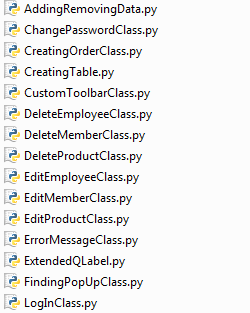
\includegraphics[width=\textwidth]{./FilesExample.png}
\end{figure}

The Above does not show the structure of my code as such, however it shows that i have seperated each class into its own individual file. I have split each class into its own file as this made it a lot easier when trying to debug problems with my code. For example if i know there was something wrong with Editing a Product, i would instantly know that i would have to look at EditProductClass.py . This made finding problems in my code very easy compared to if i had grouped many classes into one file. It also helped to shorten the length of each file, which means the contents of each file can be organised a lot easier.

\subsection{Table used for the Search Window}
\begin{figure}[H]
\pythonfile[firstline=66, lastline=71]{./Maintenance/AddingMemberClass.py}
\end{figure}

The above code shows how the County ComboBox is populated. During the Implementation stage i know it would be very long and tedious, hard coding each and every county in the UK into the ComboBox. Therefore, i created a text file containing all the counties, each separated with a comma. From here i could use python to extract each county from the text file and add it to a list. Line 70 from the code above shows a FOR loop, which places each item into the ComboBox. Using a For loop allowed me to reduce the amount of code compared down to 2 lines, compared to hard coding each county into the Combobox. 

\subsection{Emailing Functionality}
\begin{figure}[H]
\pythonfile[firstline=650, lastline=674]{./Maintenance/Main.py}
\end{figure}

The above code shows the exception handling when trying to send an email. I have used exception handling for common errors that occurred during the implementation stage when trying to send emails. The two common errors i had when trying to send emails was the credentials used to send the email were not valid, and not being connected to the Internet. If either of these problems occur, the user is now displayed with an appropriate message telling them why the email could not be sent. I also included a third except statement that will cover any other problems that may occur when sending an email, however there is no way to specify to the user what the problem is. Putting these except statements in greatly reduced the chance of my system to break when being used.

\subsection{Validation Function}
\begin{figure}[H]
\pythonfile[firstline=256, lastline=260]{./Maintenance/AddingMemberClass.py}
\end{figure}

The function above shows how the Members Postcode is validated. In order for the postcode to be valid, the text entered by the user must match the regular expression for the postcode. Using a regular expressions allows many different postcodes to be valid, without having to specify exactly which postcodes are valid. For example saying that the exact postcode 'CB7 5LQ' is avalid as apposed to saying : "if the postcode starts with 2 letters followed by a number then it is valid. This section of code is a Function because it reduces the repetition of code and gets called every single time the text in the postcode field is changed. 

\pagebreak

\section{Variable Listing}

You can find my data dictionary on Page 104 
\begin{center}
    \begin{tabular}{|p{1.5cm}|p{4.5cm}|p{1.5cm}|p{3cm}|}
        \hline
        \textbf{Variable Name} & \textbf{Purpose} & \textbf{Section} & \textbf{Line Numbers}\\ \hline
	self.title & The Text that is displayed at the top of each Interface & Main Program & 108, 115, 129, 145, 159, 172, 186, 202, 214, 226, 238, 251 \\ \hline
	\multirow{3}{*}{encrypted-password} & \multirow{3}{*}{stores the password after it has been encrypted} & Main Program & 678, 719, 762 \\ 
	& & SQL Queries & 233, 242, 244, 535 \\
	& & Preferences & 166 \\ 
	self.valid & is a boolean variable to say whether a method returns true or false. & Main Program &  774 \\ \hline
	subject & used to store the Subejct of the email that is sent to the customer / employee & Main Program & 797 \\ \hline
	send-from & used to store the email address the email is sent from & Main Program & 799, 820 \\ \hline
	self.code & The random 4 digit code that is generated when an Employee wants to reset their password. & Main Program & 818 \\ \hline
	employee-info & stores the information about an employee so that it can be used in an email. I.e the password reset email says: Hello ... where ... is the name of the employee. & Main Program & 822 \\ \hline
	self.spacer & used to add spacing between widgets & & \\ \hline
	self.vertical-spacer& used to add vertical spacing between widgets & & \\ \hline
	first-name & used to store the first name entered by the user & Main Program & 778 \\ \hline
	last-name & used to store the last name entered by the user & & \\ \hline
	full-name-list & Used to store the First letter of the First Name, The last name and the EmployeeID. & & \\ \hline
	self. pattern & used as a variable for the regular expressions used in the validation & & \\ \hline
	self. postcode-input & used to store a postcode to check if the postcode is i the CSV file. & & \\ \hline
	self. county-list & A list used to  store all the counties in the UK & & \\ \hline
	self. scaled-image & a a variable used to store a QPixmap that has been scaled to a specific width and height & & \\ \hline
	path & used to store the path of the Product Image selected by the user & & \\ \hline
	rows- in-table & used to store the amount of rows currently in a table & & \\ \hline
	self. file-name & used to store the New ProductID of the image going to be stored. & & \\ \hline
	self. temp & used to store a temporary value & & \\ \hline
	self. category-string & used to turn the combobox selection by the user into string. For example if the user selected Dog and Food from the combo-boxes, self. category-string would store the string 'Dog Food'.& & \\ \hline
	Product & used to store a list of all the Product information & & \\ \hline
	order -info & used to store a string of all the information related to an order & & \\ \hline
	data & variable used to turn individual variables into a tuple. & & \\ \hline
	date -stored & variable used to store the last sales date from the settings table & & \\ \hline
	date & used to  todays current date & & \\ \hline
	date -time & stores the current time in hours and minutes & & \\ \hline
	invoice -date & stores the date the invoice was created & & \\ \hline
	new -date & stores the todays date + 7 days (1 week) & & \\ \hline
	greatest -employee-id & stores the highest EmployeeID in the database & & \\ \hline
	new -employee-id & adds 1 to the highest EmployeeId to create a new EmployeeID & & \\ \hline
	move -list & stores the ProductID of all the products with a stock in Location 1 less than 5 & & \\ \hline
	restock -list & stores the ProductID of all the products with a stock in Location 1 and Location 2 less than 5. & & \\ \hline
	total -stock & adds the stock in Location 1 to the stock in location 2 and stores this value. & & \\ \hline
	self. subtotal-price & adds the prices of all the Products currently in the order and stores this value.& & \\ \hline
	self. total-price & stores the value from (self.subtotal-price - self.discount) & & \\ \hline
	self. money-off & calculates (self .total-stock * 0.1) and stores the value & & \\ \hline
	invoice -history & is an array that stores the date and time the invoice was made and the date and time the invoice was sent & & \\ \hline
	html & used to store the HTML invoice that is either printer or emailed to a customer& & \\ \hline
	\end{longtable}
\end{center}
	
	
	


\section{System Evidence}

\subsection{User Interface}

\begin{figure}[H]
    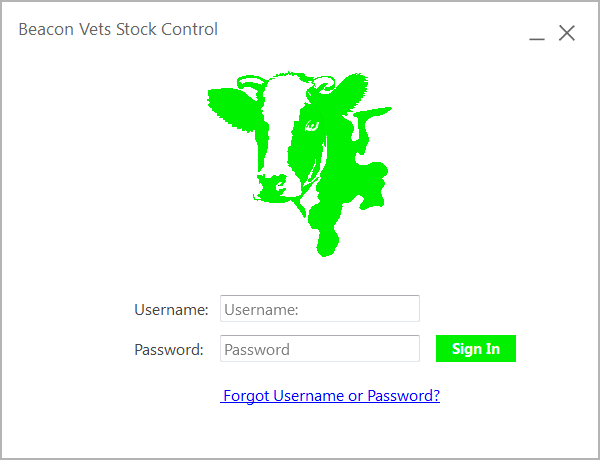
\includegraphics[width=\textwidth]{./interface1.png}
    \caption{Logo In Interface} \label{fig:log-in-interface}
\end{figure}

Figure \ref{fig:log-in-interface} is my log in interface. The figure below shows the Widgets and Layouts used to create the log in interface. 

\begin{figure}[H]
    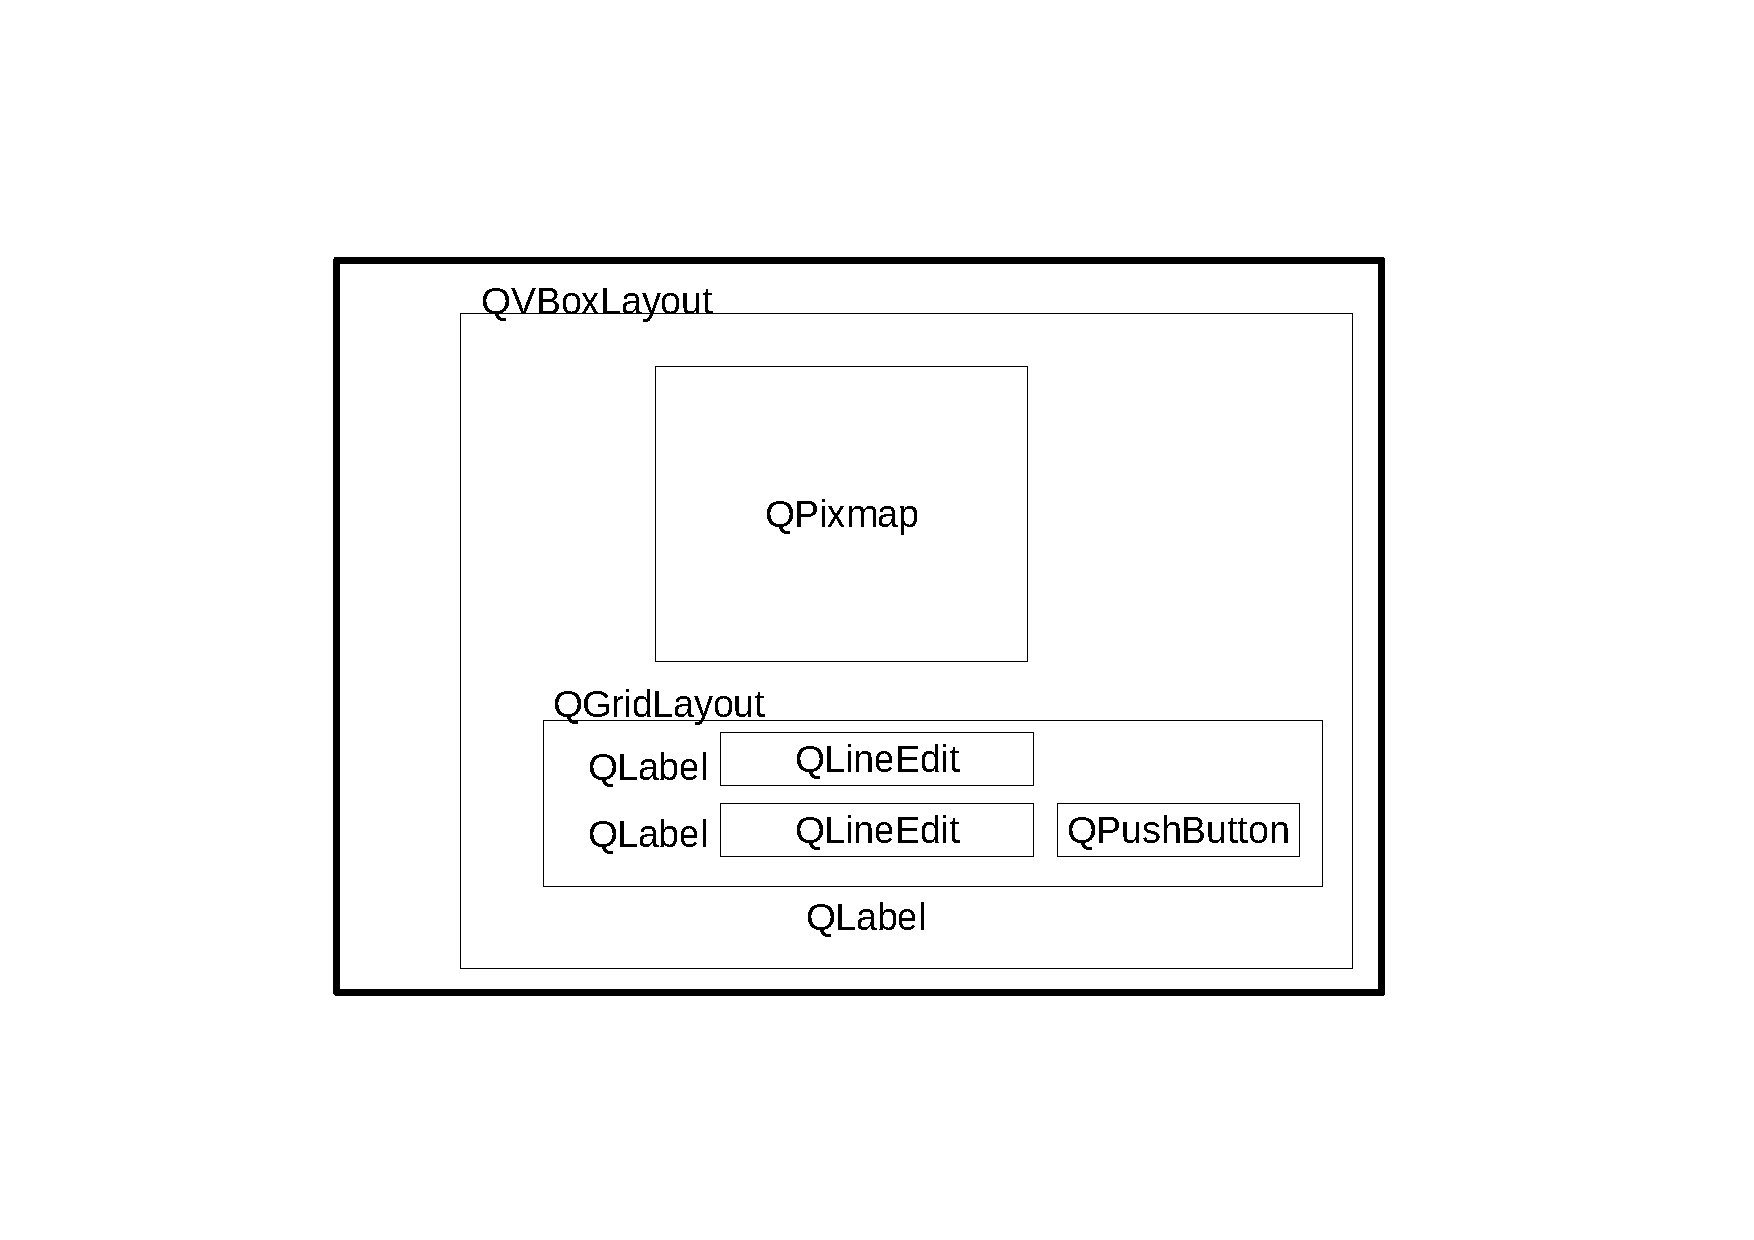
\includegraphics[width=\textwidth]{./structure-log-in.pdf}
    \caption{Structure of the Log In Interface} \label{fig:log-in-structure}
\end{figure}

The Log in Interface is built up from many widgets. The QPixmap is the logo of the company, The QLabels within the Grid layout tell the user what to enter into the QLineEdits. The QPushButton is the button in whihc the user presses once they have entered their log in details. If The user forgets their account details they can click on the Forgot Password Label which is the QLabel underneath the QGridLayout.

\begin{figure}[H]
    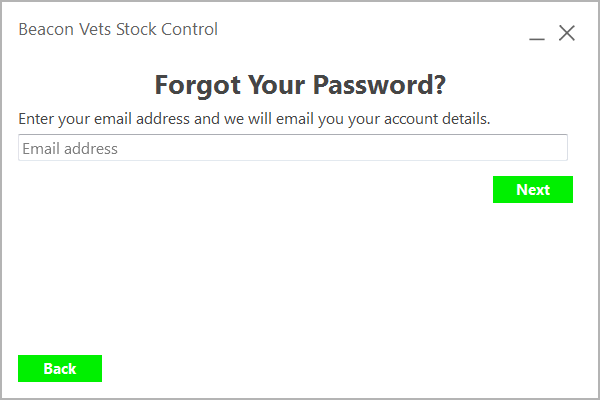
\includegraphics[width=\textwidth]{./interface2.png}
    \caption{Forgot Password Interface} \label{fig:forgot-password-interface}
\end{figure}

The forgot password interface has a QLabel with a unique style sheet that makes the text size larger and makes the text bold. This QLabel is the text that says: `Forgot Your Password.' This same style sheet has been used for all the other titles on each interface to tell the user what interface they are currently on. The forgot password interface then has a QLabel telling the user what to enter into QLineEdit. There is a QLineEdit in which the user can enter their email address and a QPushButton in which the user can click when they have entered their password. When the button has been clicked the database is searched for the email address the user entered. There is also a QPushButton in the Bottom left hand corner of the interface which the user can click to go back to the log in interface. This QPushButton was positioned in the bottom left corner using spacers which are just QWidgets that cannot be seen by the user.


\begin{figure}[H]
    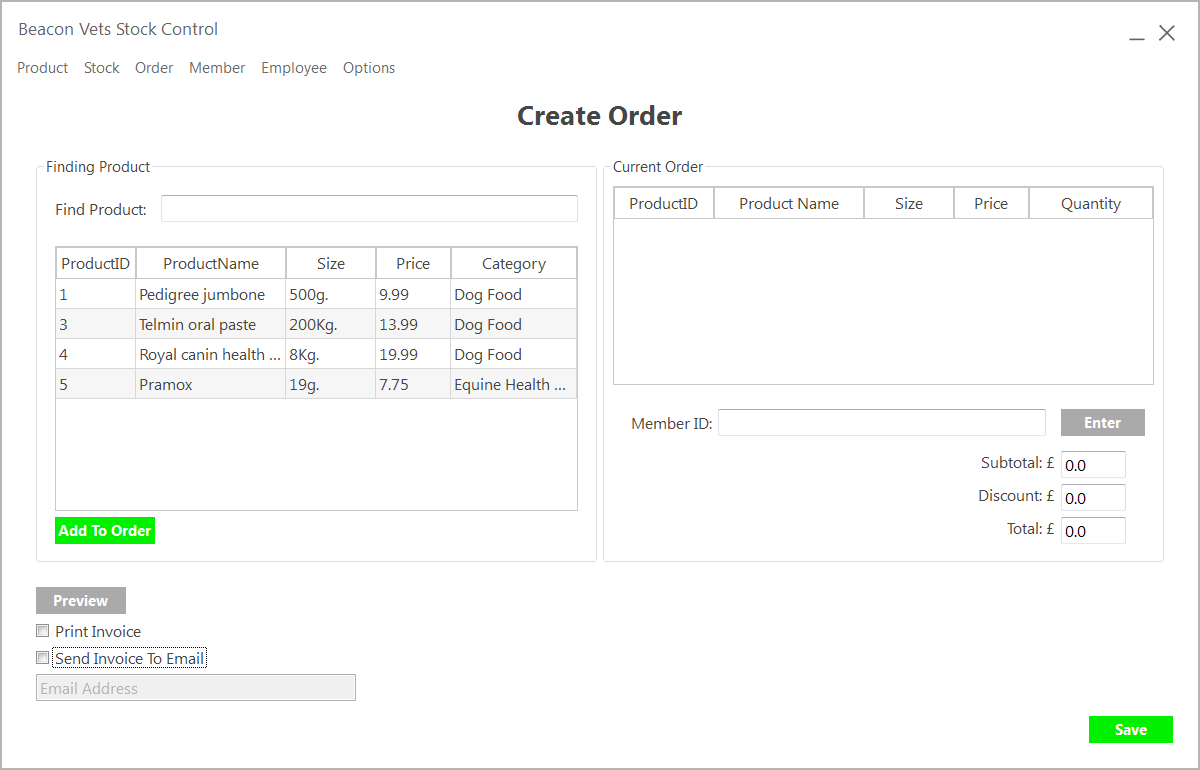
\includegraphics[width=\textwidth]{./interface3.png}
    \caption{Creating Order Interface} \label{fig:creating-order-interface}
\end{figure}

The create order interface was the most complex interface to design as it had to include many more widgets, compared to the other interfaces. below i have provided a diagram of all the widgets and layouts used to create the create order interface.

\begin{figure}[H]
    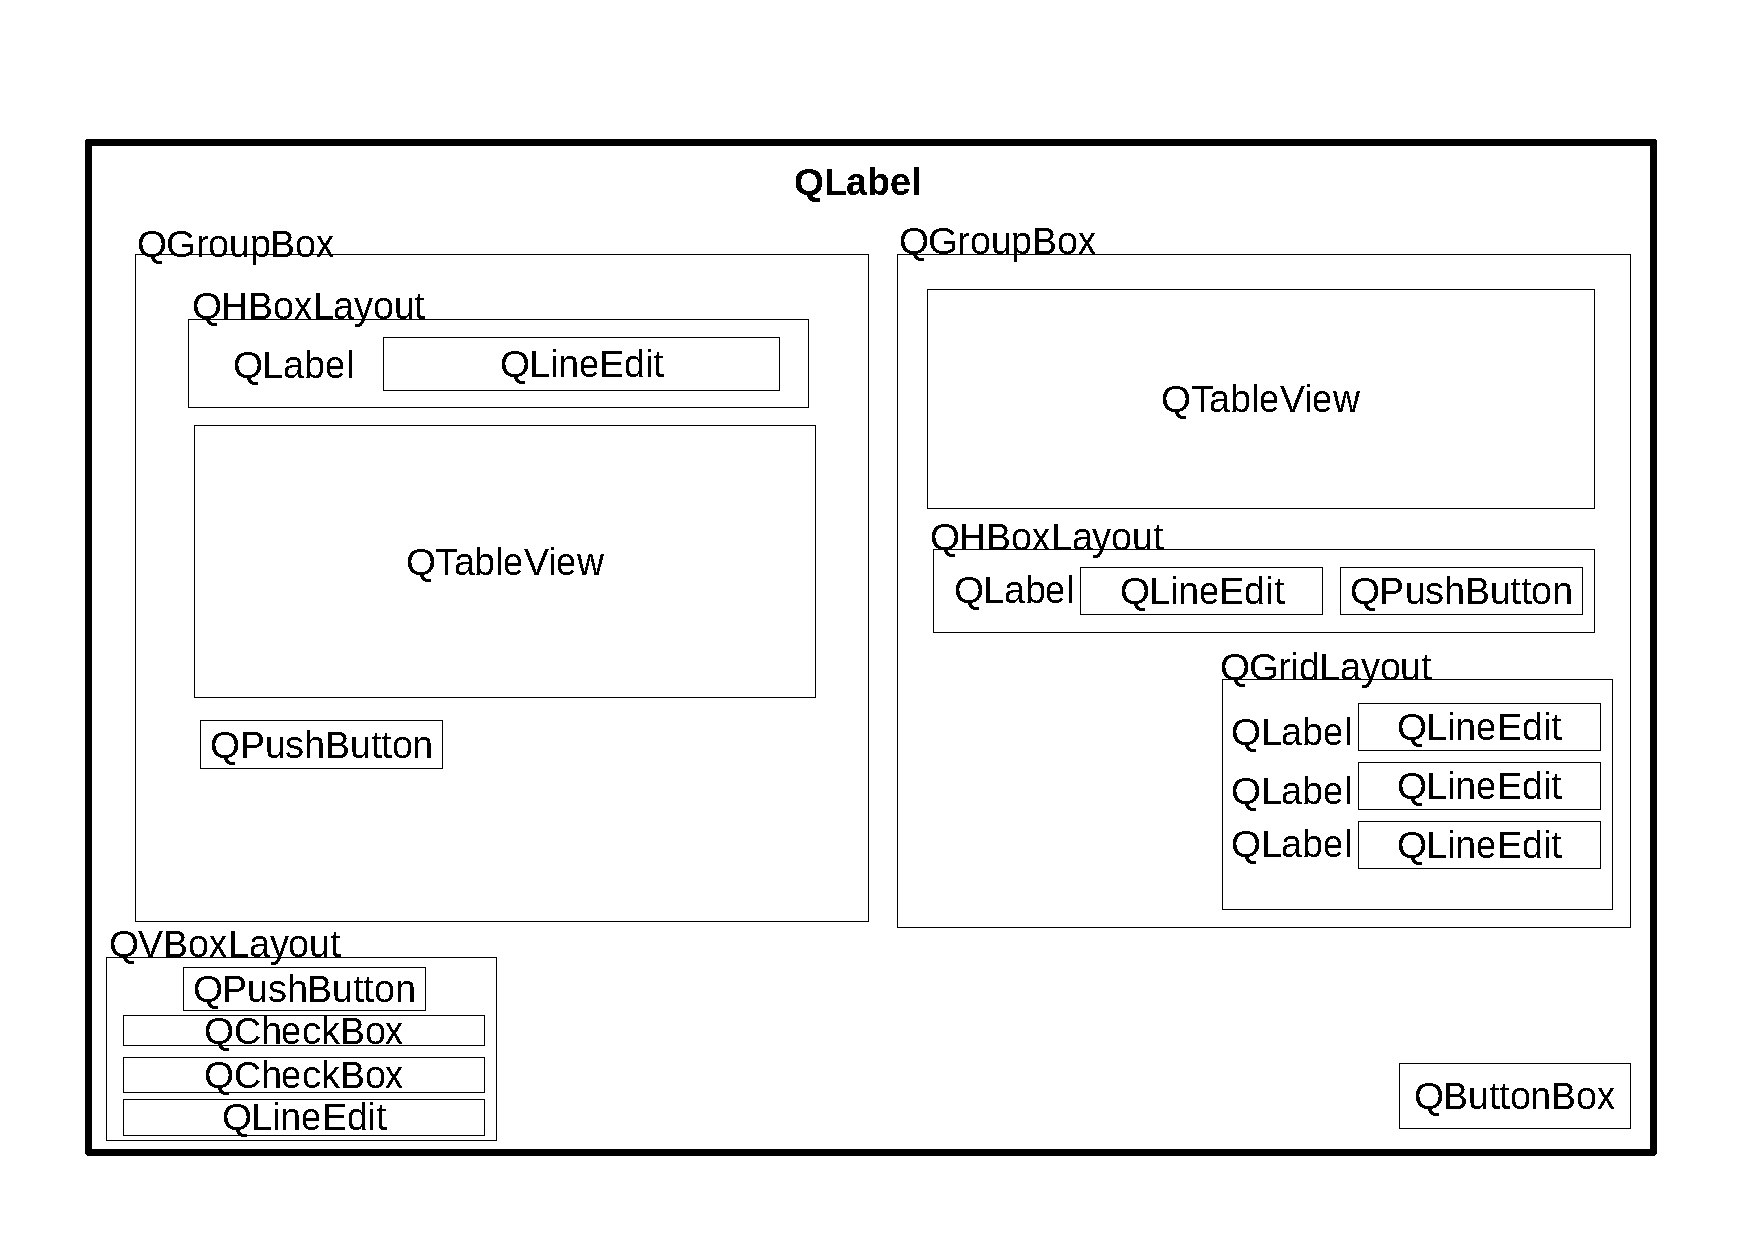
\includegraphics[width=\textwidth]{./structure-order.pdf}
    \caption{Structure of the Order Interface} \label{fig:structure-order}
\end{figure}

The QLabel in bold at the top of the page is the title of the page. This QLabel has a unique stylesheet as explained before, which gives the text are larger font and is in bold. The QGroupBox on the left is for the user to find a product. the QTableView in this QGroupBox displays the Product Table from the database. If the user enters any any characters into the QLineEdit within this group box, the system searches the Product Table for whatever the user entered and will display it in the table. This allows the user to search for specific products. The QPushButton in the QGroupBox will allow the user to add a specific product to the order if they have selected one in the table. Alternatively, the user can double click on a product in the table. The QGroupBox on the right is for the current order. the QTableView displays all the products that are currently in the order. When a user adds an item from the Product Table to the order, that product should be displayed in the current order table. Members get a 10 percent discount, therefore, there is a field that allows the user to enter a member id and the system will deduct 10 percent of the total price from the subtotal. The QLabels and QLineEdits in the QGridLayout display to the user; the subtotal of the order, the amount of money the customer gets off due to discount and the final price of the order after discounts. At the bottom of the page is where the user can decide how they want to output the invoice. The QPushButton allows the user to preview the invoice to ensure all the products have been added successfully. The two QCheckBoxes allow the user to either print the invoice, send it to an email or both. The QLineEdit in this QVBoxLayout allows the user to enter the email address to send the email to. The QButtonBox contains the save button where the user can save the Order to the database and they invoice can be printed or emailed.

\begin{figure}[H]
    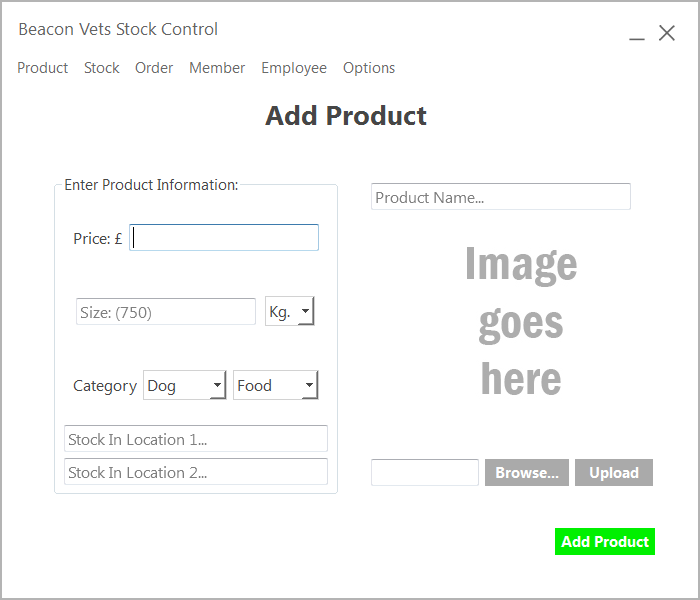
\includegraphics[width=\textwidth]{./interface4.png}
    \caption{Add Product Interface} \label{fig:add-product-interface}
\end{figure}

The Add Product interface contains 6 QLineEdits. 5 of the QLineEdits are for the Employee to enter the product information and one is for displaying the image path to the user. The QLineEdit for displaying the image path has been set to Read Only so that the user cannot edit the path. The QLineEdits for the data inputs allow the user to enter letters, numbers and special characters. After creating my system, i feel it would have been more sensible to use QSpinBoxes for the stock inputs as these only allow integers to be entered into the field. I have used some QLabels to tell the user what to enter into the field, however this is also done by the place holder text within the QLineEdits. I have used two QPushButtons, one allows the user to search for the image, the other updates the QPixmap so that it displays the image selected to the user. The QPushButton in the bottom right corner allows the user to save the product. Once they have entered data into all the fields they can click this button to add the product to the database.


\begin{figure}[H]
    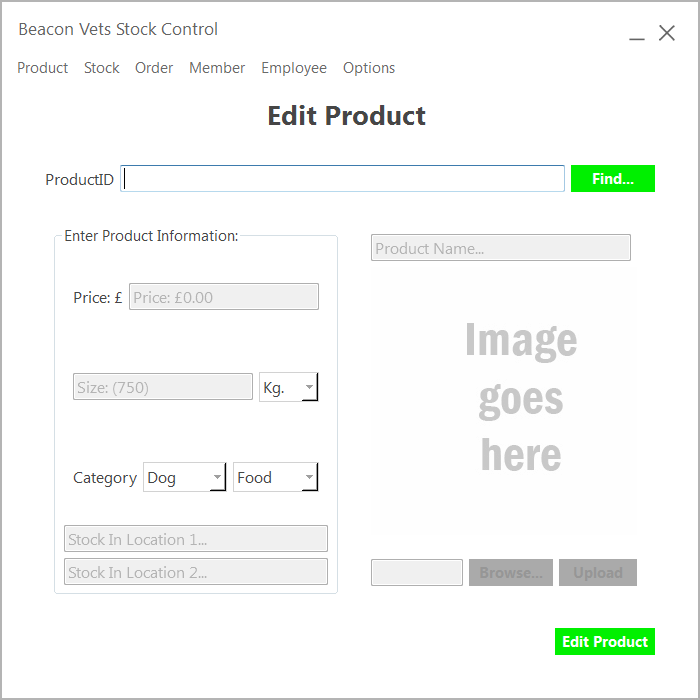
\includegraphics[width=\textwidth]{./interface5.png}
    \caption{Edit Product Interface} \label{fig:edit-product-interface}
\end{figure}

The Edit product interface is similar to the add product interface however there is an additional widget between the title and the main widget. The additional widget is a QLabel, QLineEdit and QPushButton in a QHBoxLayout. The QLabel tells the user what data needs to be entered into the QLineEdit (ProductID), and the QPushButton searches the database for the data the user enters. Until a Product has successfully been found, all the widgets inside the main widget have been disabled which means the user cannot enter data into them. The Edit Product push button has also been disabled.
\begin{figure}[H]
    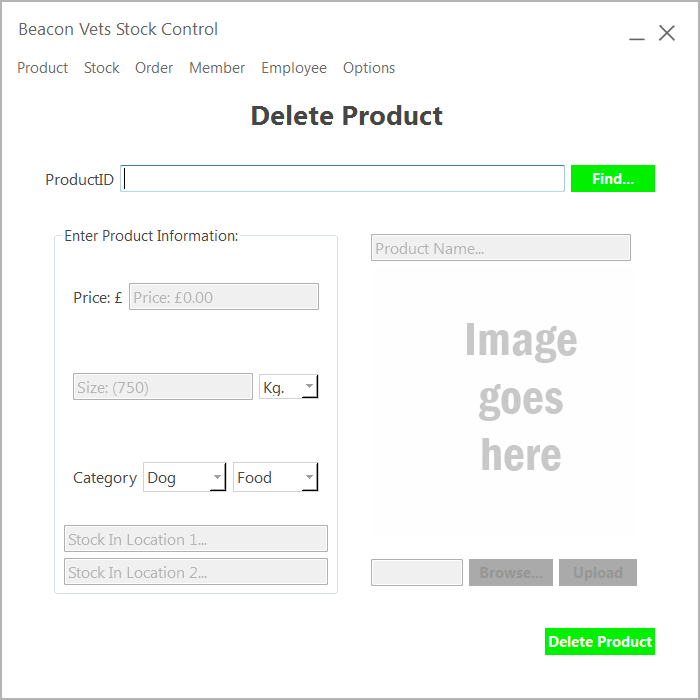
\includegraphics[width=\textwidth]{./interface6.png}
    \caption{Removing Product Interface} \label{fig:removing-product-interface}
\end{figure}

Visually, the Edit and Delete Product interfaces look extremely similar. however there are some slight differences in their functionality. Once the user has found a product, in the Delete Product interface, the data fields are set to read only. This means the user cannot edit the data in the data fields. Also, when the user finds a product in the delete member field, no validation takes place because no data is being changed and the data should have been valid when it was input originally. When the user clicks the delete product push button, the system searches for the product id and removes it from the database.

\begin{figure}[H]
    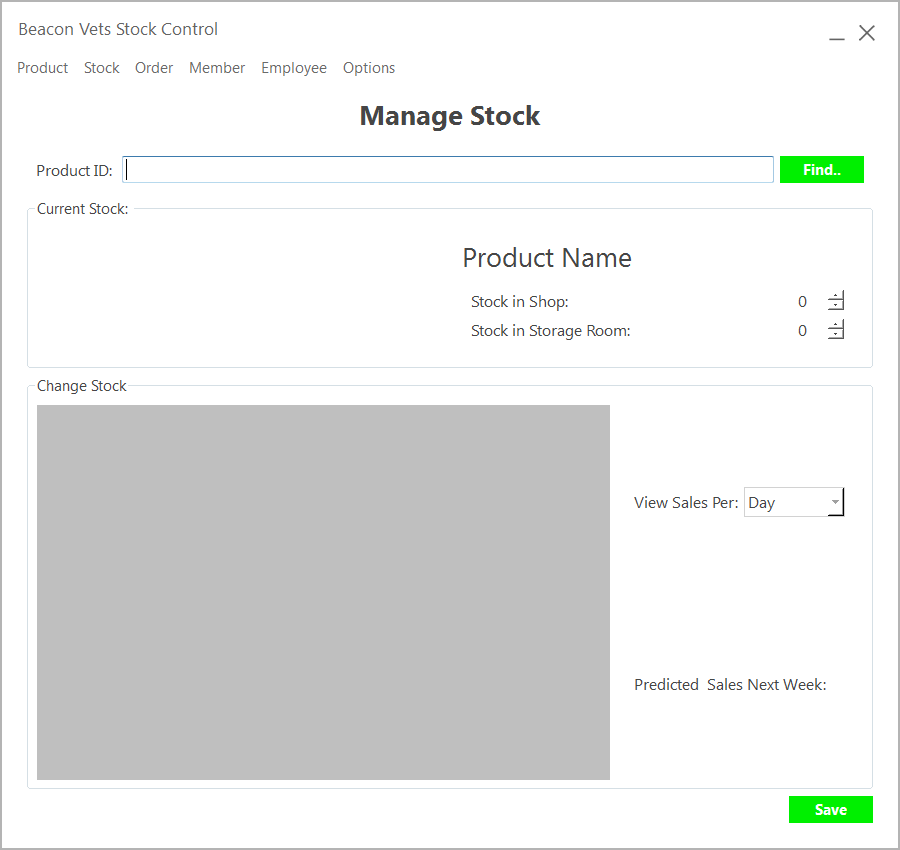
\includegraphics[width=\textwidth]{./interface7.png}
    \caption{Manage Stock Interface} \label{fig:stock-interface}
\end{figure}

The Manage stock interface contains three widgets inside a QVBoxLayout. There is the Widget in which the user enters the ProductID of the Product they want to edit the stock of, The Current Stock groupbox which shows the current stock of the product in the database, along with displaying the product name and product image to ensure the user is editing the stock of the correct product. The Other GroupBox shows the sales of that product over a period of time. The graph displays the amount of sales made on a specific date. Inside this GroupBox there is a QComboBox that allows the user to change the graph to show either the sales made each day, or sales made each week. The graph also works out the predicted sales for the following week, which is output to the user in a QLineEdit that is set to Read Only. The save button in the QButtonBox allows the user to save the new stock if they changed it.

\begin{figure}[H]
    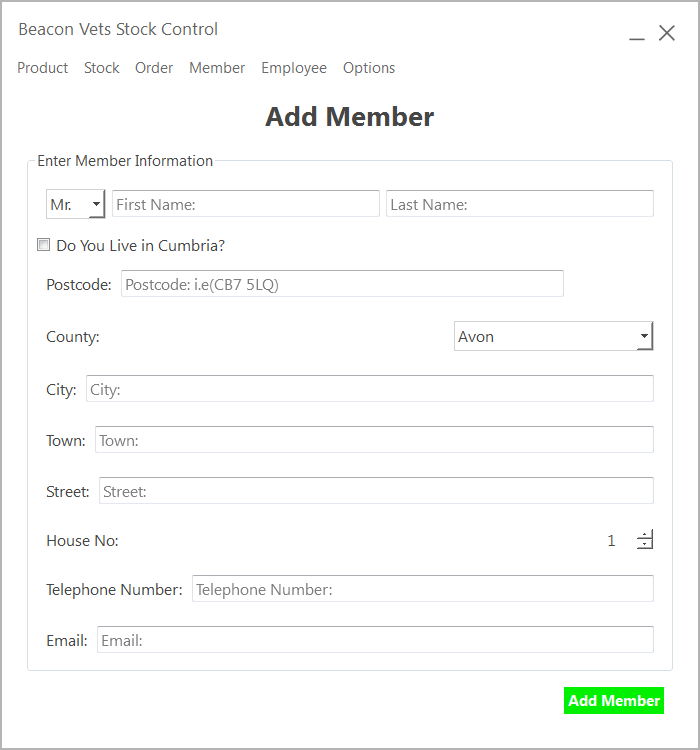
\includegraphics[width=\textwidth]{./interface8.png}
    \caption{Add Member Interface} \label{fig:add-member-instance}
\end{figure}

The Add Member interface has many QLineEdits, in which the user enters data about the Member. A QComboBox has been used for the Title (i.e Mr. or Mrs), and the county. The House Number field is a QSpinBox as the only allows the user to enter an integer. The state of the QCheckBox depends on whether a QPushButton is displayed. If the user does live in Cumbria, the user can click the checkbox which will cause a push button to appear. clicking this push button will search a CSV file containing all the postcodes and towns of all the postcodes in Cumbria. If the postcode is in the database the county and town field will be filled out automatically. This is to decrease the amount of time the user must spend to physically type information into the system.


\begin{figure}[H]
    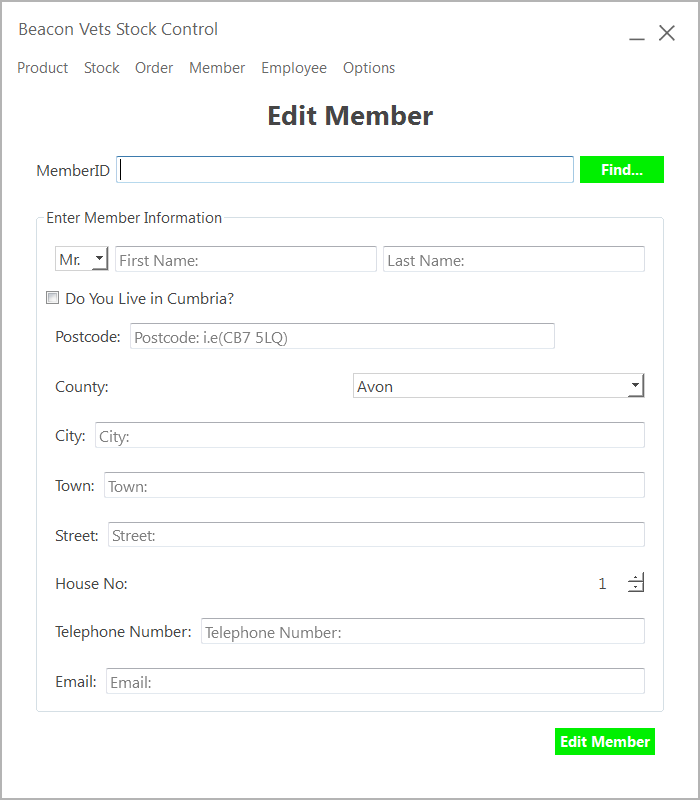
\includegraphics[width=\textwidth]{./interface9.png}
    \caption{Edit Member Interface} \label{fig:edit-member-instance}
\end{figure}

The Edit Member interface is very similar to the add member interface however it has a widget between the Title of the interface and the main widget. The new widget contains a QLabel that tells the user what to enter into the QLineEdit, a QLineEdit where the user enters the Member ID and a QPushButton, that when pressed, searches the database for a MemberID that matches the MemberID entered by the user. 

\begin{figure}[H]
    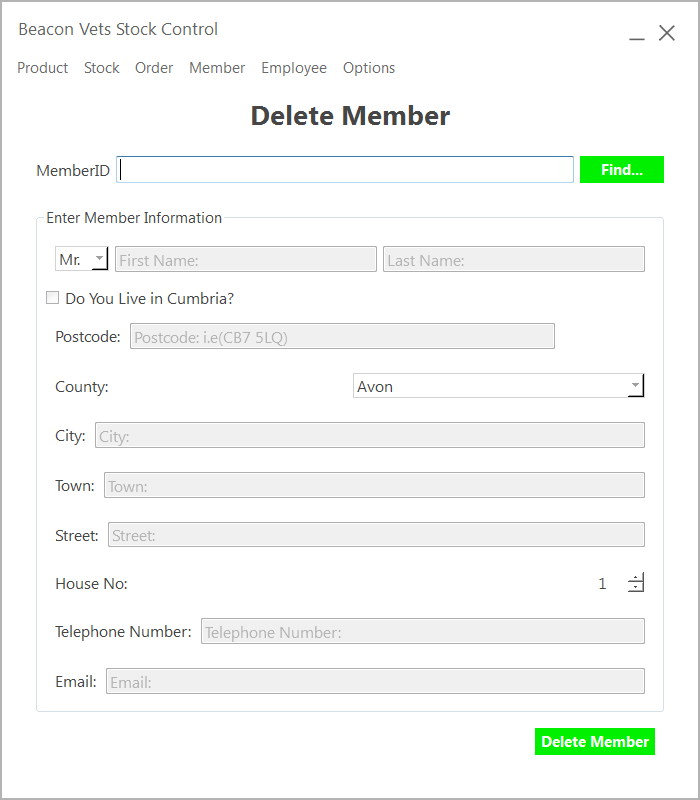
\includegraphics[width=\textwidth]{./interface10.png}
    \caption{Removing Member Interface} \label{fig:removing-member-interface}
\end{figure}

The Delete Member interface is visually identical to the Edit Member interface, other than the text on the QPushButton in the bottom right hand corner of the interface. When the Delete Member button is clicked, the system searches the database for the MemberId entered by the user and is removed from the system.

\begin{figure}[H]
    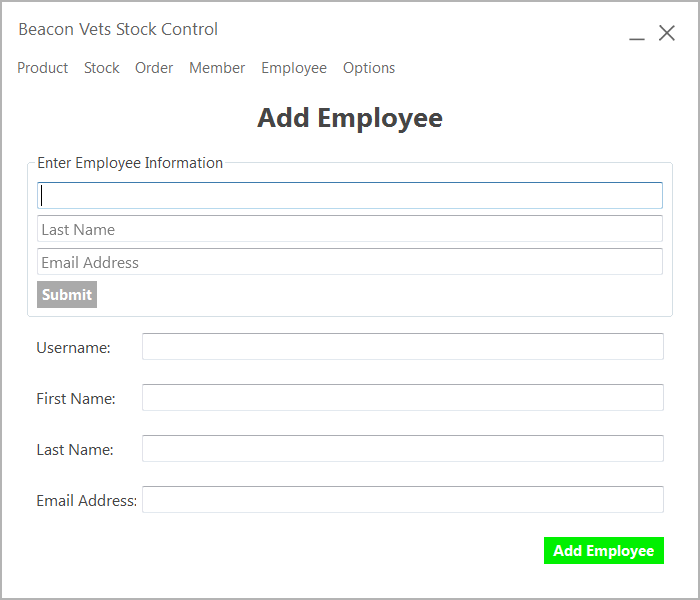
\includegraphics[width=\textwidth]{./interface11.png}
    \caption{Add Employee Interface} \label{fig:adding-employee-interface}
\end{figure}


\begin{figure}[H]
    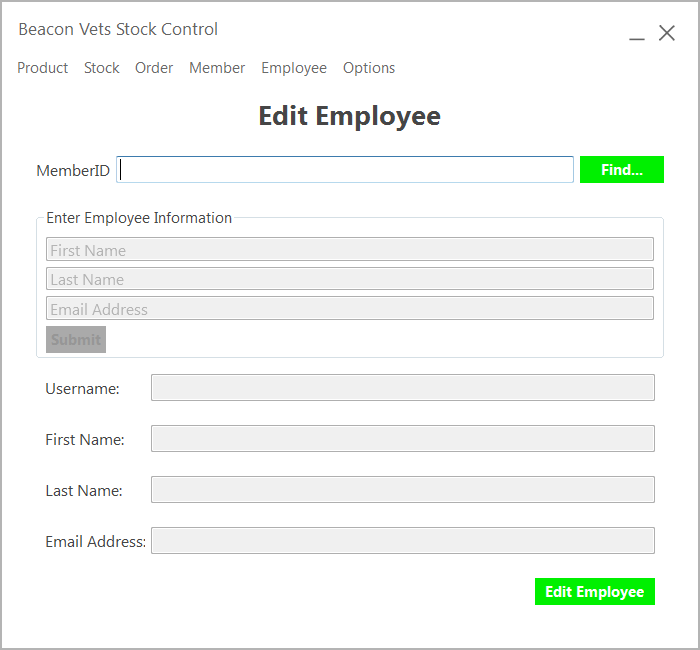
\includegraphics[width=\textwidth]{./interface12.png}
    \caption{Edit Employee Interface} \label{fig:edit-employee-interface}
\end{figure}

\begin{figure}[H]
    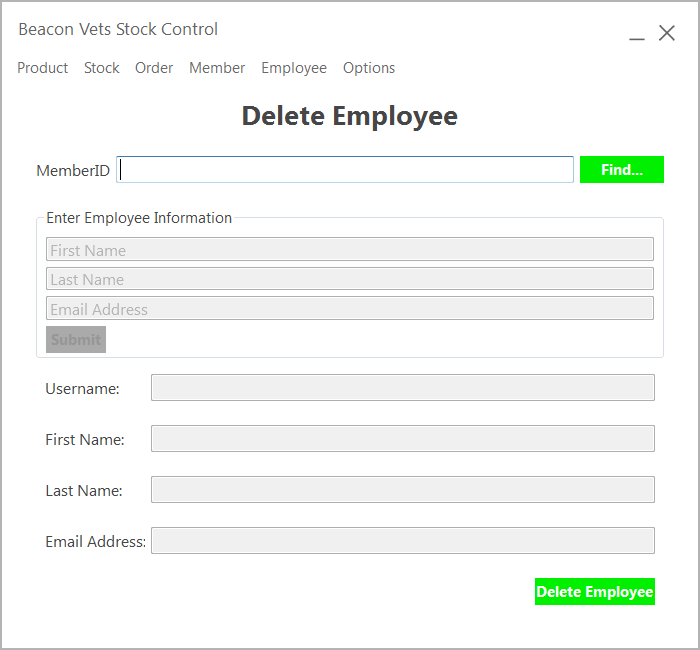
\includegraphics[width=\textwidth]{./interface13.png}
    \caption{Remove Employee Interface} \label{fig:removing-employee-interface}
\end{figure}

\begin{figure}[H]
    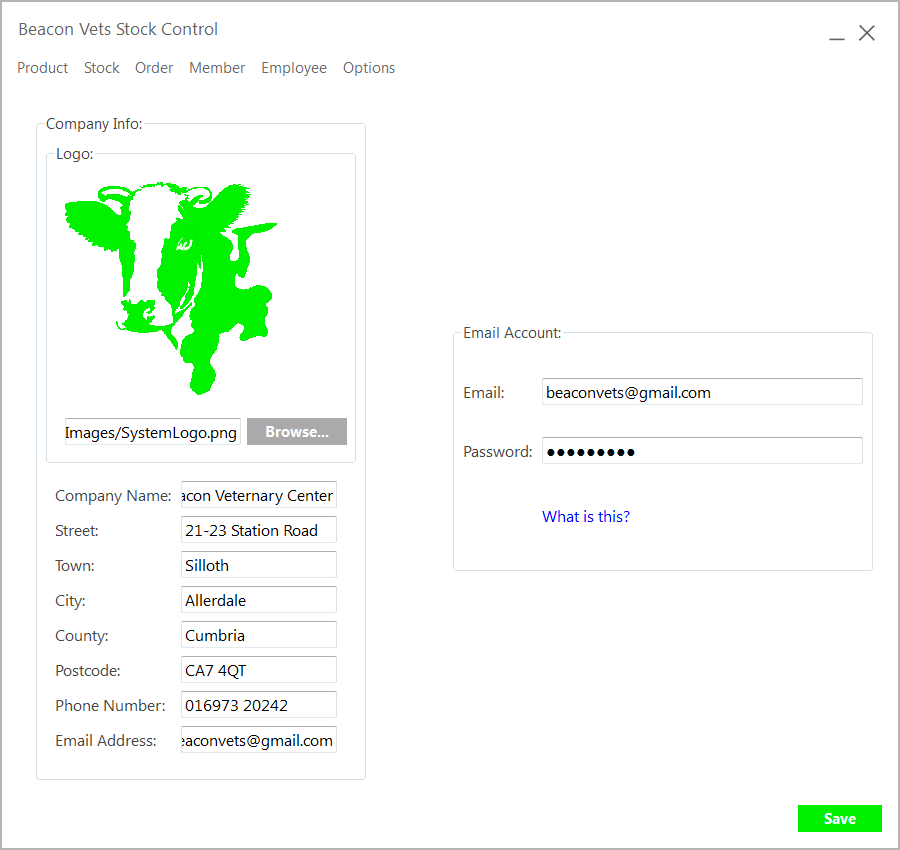
\includegraphics[width=\textwidth]{./interface14.png}
    \caption{Preferences Interface} \label{fig:preferences-interface}
\end{figure}

\begin{figure}[H]
    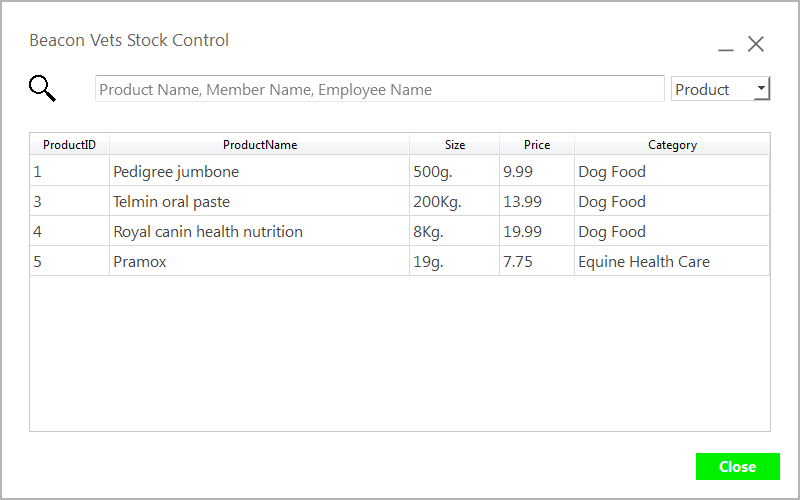
\includegraphics[width=\textwidth]{./interface15.png}
    \caption{Search Interface} \label{fig:search-interface}
\end{figure}

\begin{figure}[H]
    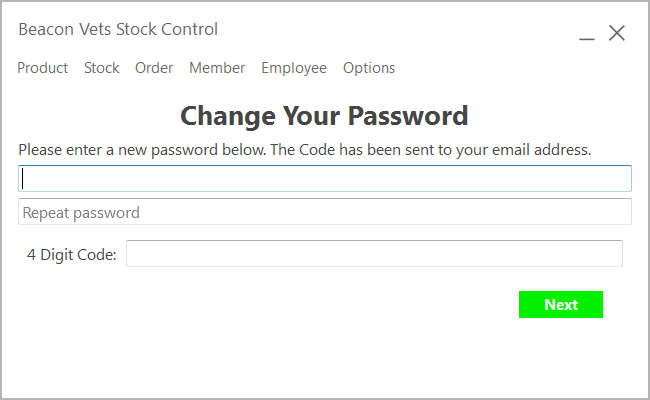
\includegraphics[width=\textwidth]{./interface16.png}
    \caption{Change Password Interface} \label{fig:change-password-interface}
\end{figure}

Another aspect of the system i felt was important was the visual design of the system. One of the Objectives in my system analysis was that the system had to have a clear layout. The objectives from my analyisis can be found on page \pageref{ref:objectives}. I felt that by changing the visual appearance of the system, i could improve upon the clarity of the layout and the ease of use of the system. Currently, my client has chosen to use a white and green colour scheme the the company website, interior and exterior of the veterinary center. I have provided a screen-shot below to give a better understanding of the colour scheme of the website, for a further understanding of the colour scheme of the website, you can visit it at www.beaconvets.co.uk.

\begin{figure}[H]
    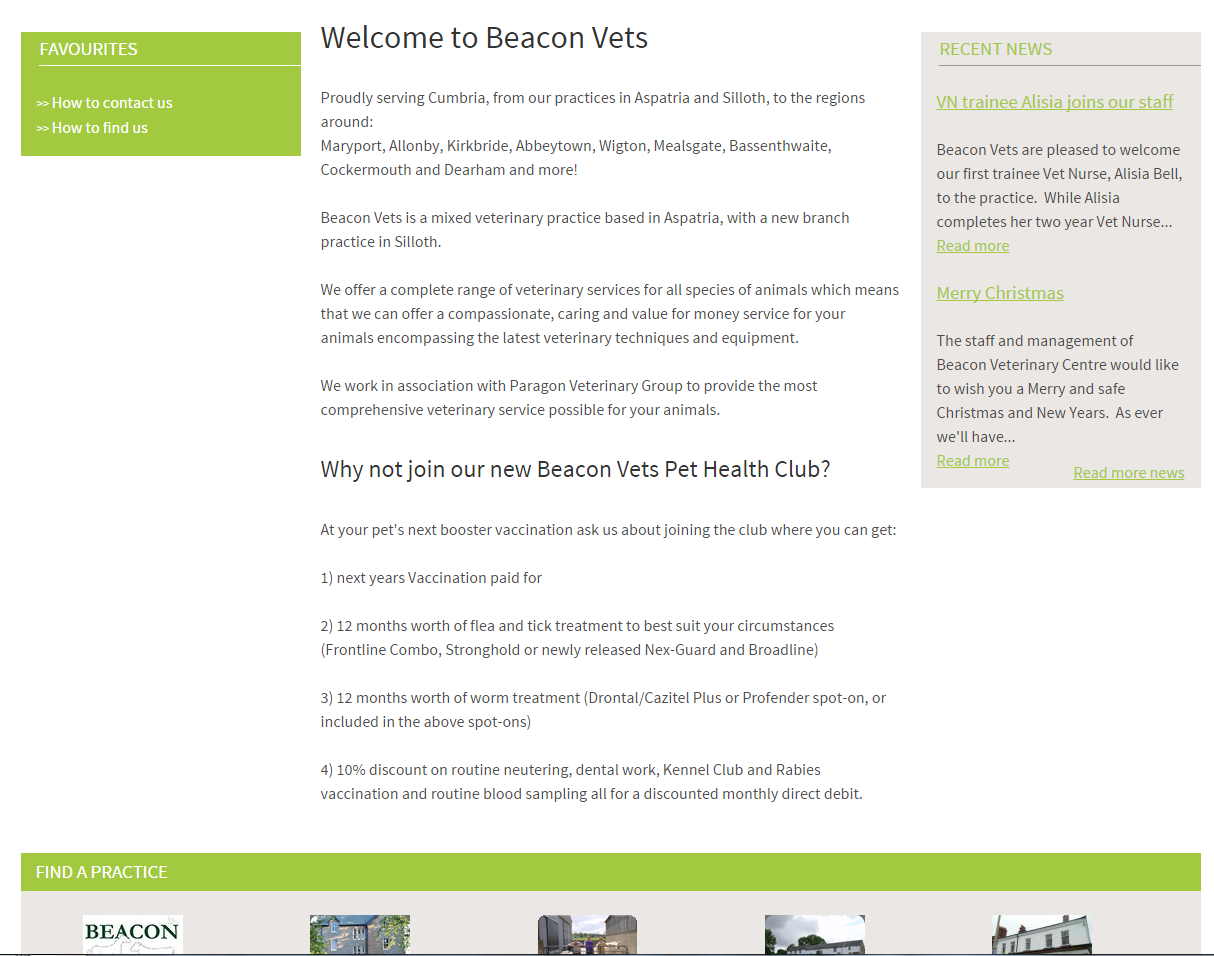
\includegraphics[width=\textwidth]{./website.png}
    \caption{Change Password Interface} \label{fig:website.}
\end{figure}

When creating the system, i wanted the system to match the colour scheme used for the other aspects of the company. Immediately, i increased the size of the font for all the text in the system as i felt that the default font size was too small to be able to read easily. I also changed the font to the 'Segoe UI' family' as i felt, this was easier for the user to read compared to the default font used for PyQt widgets. I also changed the colour of the text to a very dark gray compared to black as i felt the black text contrasted the white background too much. Below i have provided comparison between the Default font, colour and size of text in PyQt and the font, colour and text used in my system. The window on the top shows what the text would look like without changing the font and colour, the window on the bottom shows the text after the changes i made.

\begin{figure}[H]
    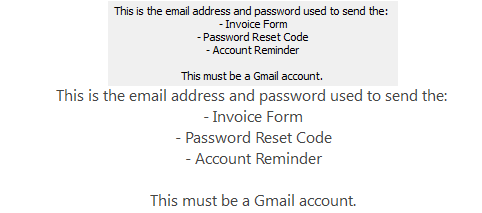
\includegraphics[width=\textwidth]{./text-comparison.png}
    \caption{Comparison between the default text, and the changes i made to the text for my system.} \label{fig:text-comparison}
\end{figure}

I investigated how to make my system easier to navigate for the user and came across Fitts's Law. Fitts's law models human movement and predicts the time it will take for the user to move to a target area such as a button. Fitts's Law is ID = log2(2A/W), where ID is the difficulty index, A is the distance to move and W is the size of the target.Therefore, to increase the ease of use of my system i had to decrease the index difficulty for the Widgets within my system. Therefore i found that one way to decrease the index difficulty was to increase the size of the targets (for example the push buttons). For the Line Edits this was the case anyway, as i had previously increased the text size anyway, which meant the line edits had to increase in size in order for the new text size to fit inside them.\par

I increased the size of the Push buttons to decrease the index difficulty, and also made the text inside the push buttons bold in order for the text to be read more easily. I decided to subtly colour code the push buttons within my system, because the colour green really stands out on the white background, i knew green push buttons would attract the users attention far better than gray push buttons. All the important push buttons within an interface were coloured green and any push buttons which were not as important, were coloured gray. Looking at figure \ref{fig:add-product-interface} on page \pageref{fig:add-product-interface}, you can see that the browse and upload image buttons have been coloured in grey and the Add product button has been coloured in green as this is the most important push button on the interface. \par

Another way to reduce the Difficulty index of the system is to decrease the distance between the current mouse position and the target area. In general to decrease this, i must decrease the size of the interface without decreasing the size of the widgets. Aswell as having problems with the layout of the widgets when the size of the window changes, i decided to make window a fixed size. This means that the window cannot be resized and the maximise button in the window title bar became redundent.

 I decided to create a custom title bar to remove the maximize button and increase the size of the minimise and close button to decrease their difficulty index too. When the minimise tool-bar is hovered it is highlighted grey, however when the close button is hovered it is highlighted bright red. This is to ensure the user does not accidentally click on the wrong button, naturally closing something is associated to the colour red, which explains my choice for this colour. During the testing stage, i definitely noticed an increase in ease of clicking the close button in the title bar before and after i implemented the custom title bar. I matched the text in the title bar to the text in the rest of the system. Below is a screenshot that shows the comparison between the title bar before and after i implemented the custom title bar. The title bar on the top is the default titlebar for PyQt widgets and the title bar on the bottom is the title bar in which i implemented into my system. 

\begin{figure}[H]
    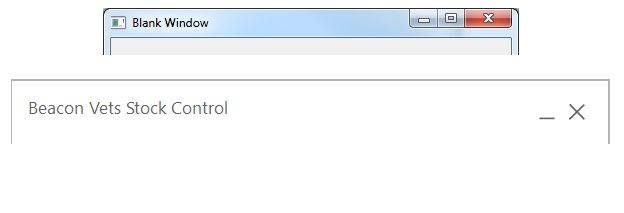
\includegraphics[width=\textwidth]{./title-bar-comparison.png}
    \caption{Comparison between the default PyQt title bar and the Title i created for my system.} \label{fig:title-bar-comparison}
\end{figure}

I Changed the text of the menu bar to match the text of the rest of the system, when a menu or option is hovered, it is highlighted in grey, i decided to change this as it found it was hard too see which option was being hovered after i changed the background colour to white. When an option is clicked it is highlighted in green, simply to match the colour scheme of the system. Below i have provided a screenshot showing the Menubar before and after i implemented the style sheet for the menubar. The menubar on the top is the Default menubar style in PyQt and the bottom menubar is the style in which i implemented in my system.

\begin{figure}[H]
    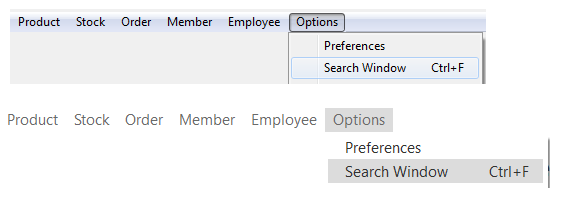
\includegraphics[width=\textwidth]{./menu-comparison.png}
    \caption{Comparison between the default PyQt menu bar and the menu bar i created for my system.} \label{fig:menu-comparison}
\end{figure}





\subsection{ER Diagram}

Since the Design stage i developed my database and added and removed some tables, that i felt needed to be changed. To see my original ER Diagram from my design, go to page \pageref{fig:ER Diagram}, figure \ref{fig:ER Diagram}. To be able to track the amount of sales made each week and each day for each product so that this data could be plotted onto a graph, i created two new entities; DailyProductSales and WeeklyProductSales, both entities take ProductID as a foreign key and i have also included a seperate table called Settings. The settings tables simple stores the preferences entered by the user and has no relationship with any of the other data. below is my new ER Diagram, i have removed Location and Product location as these Tables were not used.

\begin{figure}[H]
    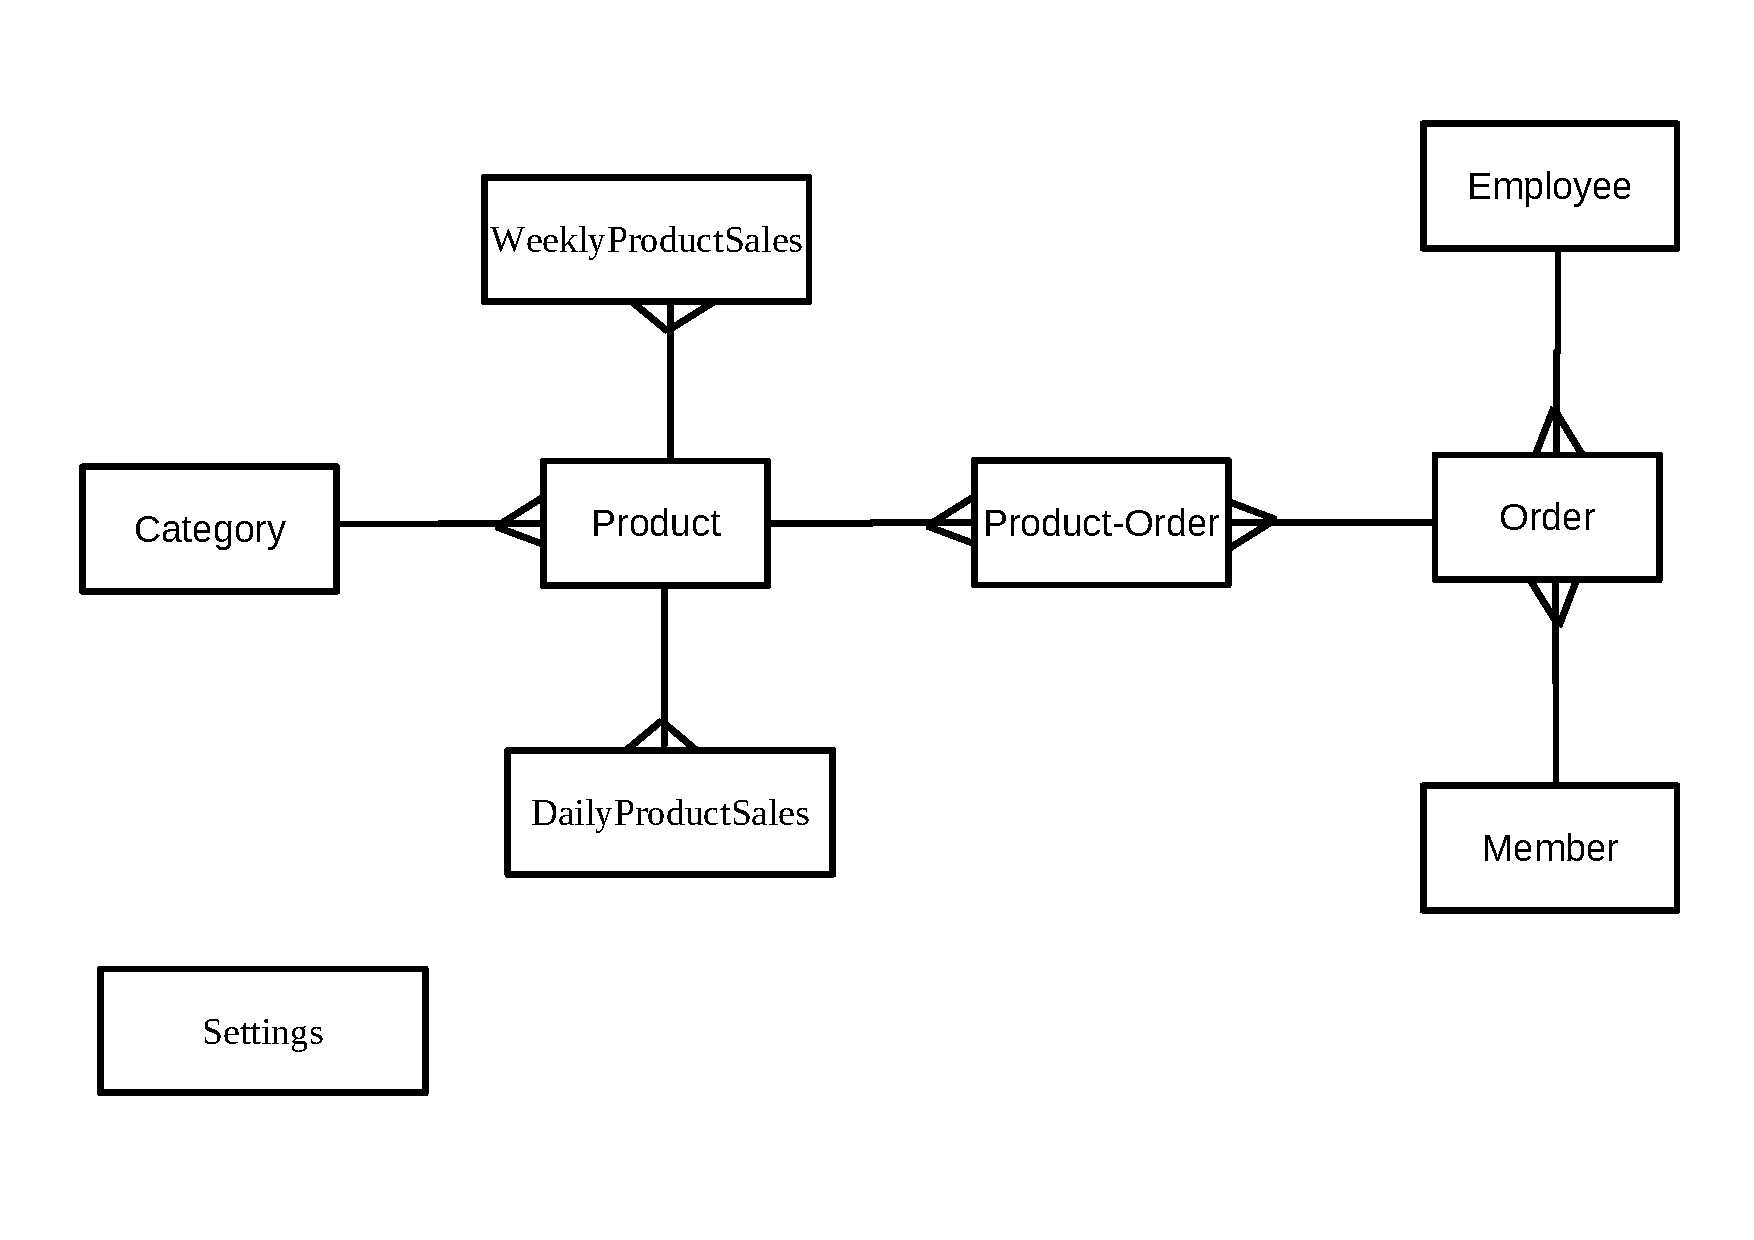
\includegraphics[width=\textwidth]{./ERDiagramMaintenance.pdf}
    \caption{New Entity Relationship Diagram} \label{fig:entity-relationship-maintenance}
\end{figure}

\subsection{Database Table Views}

\begin{figure}[H]
    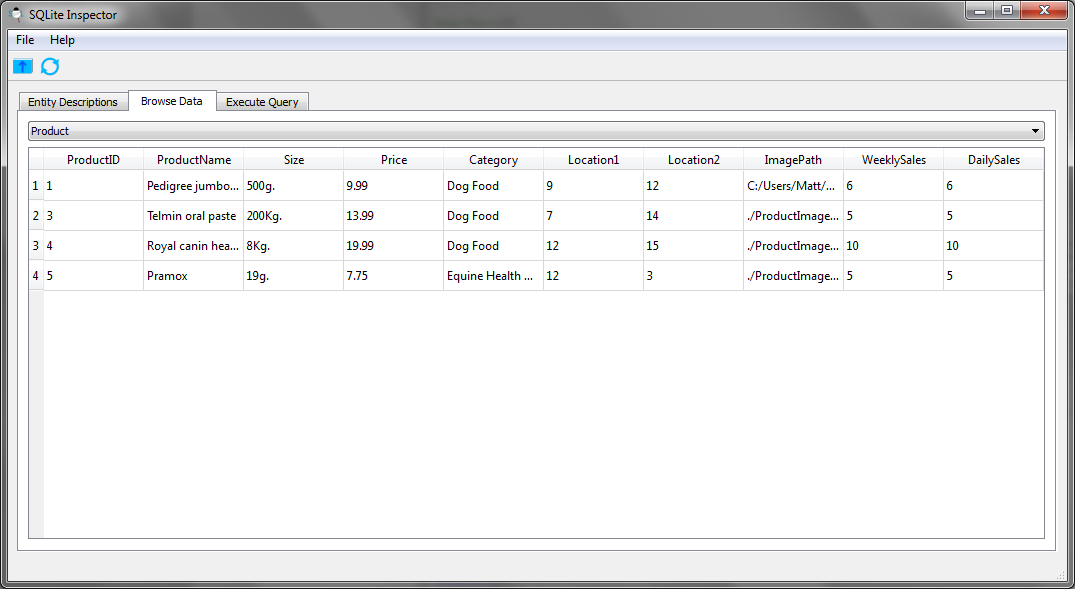
\includegraphics[width=\textwidth]{./TableView1.png}
    \caption{New Entity Relationship Diagram} \label{fig:table-view-1}
\end{figure}

\begin{figure}[H]
    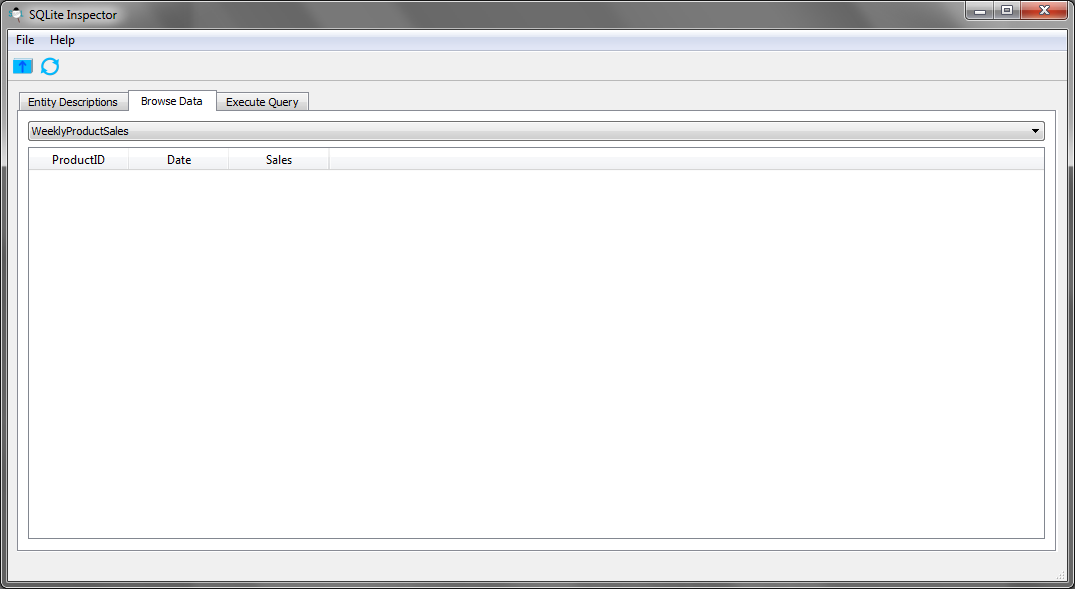
\includegraphics[width=\textwidth]{./TableView2.png}
    \caption{New Entity Relationship Diagram} \label{fig:table-view-2}
\end{figure}

\begin{figure}[H]
    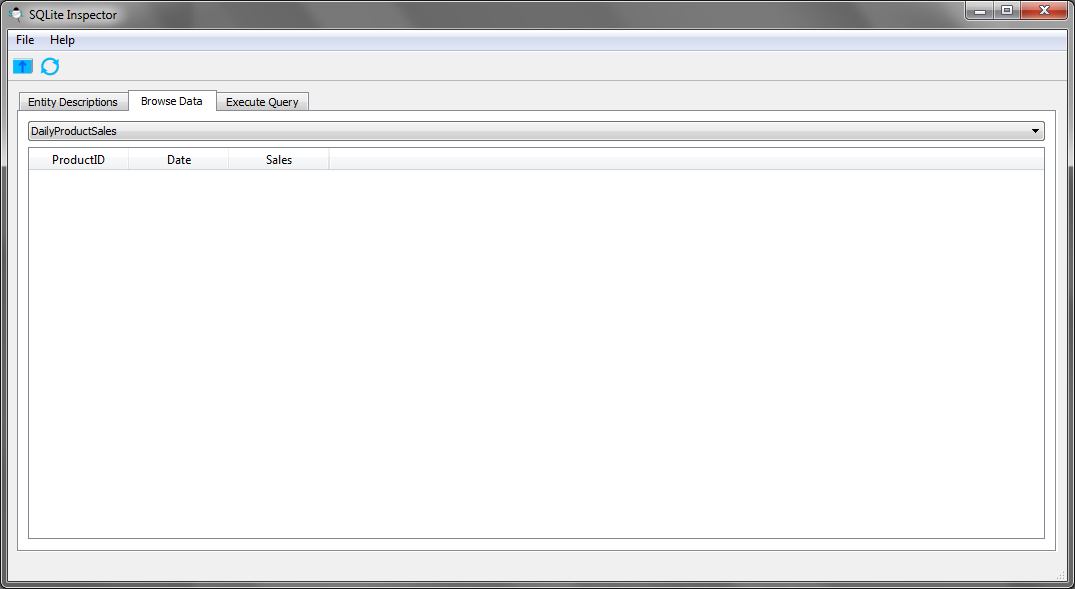
\includegraphics[width=\textwidth]{./TableView3.png}
    \caption{New Entity Relationship Diagram} \label{fig:table-view-3}
\end{figure}

\begin{figure}[H]
    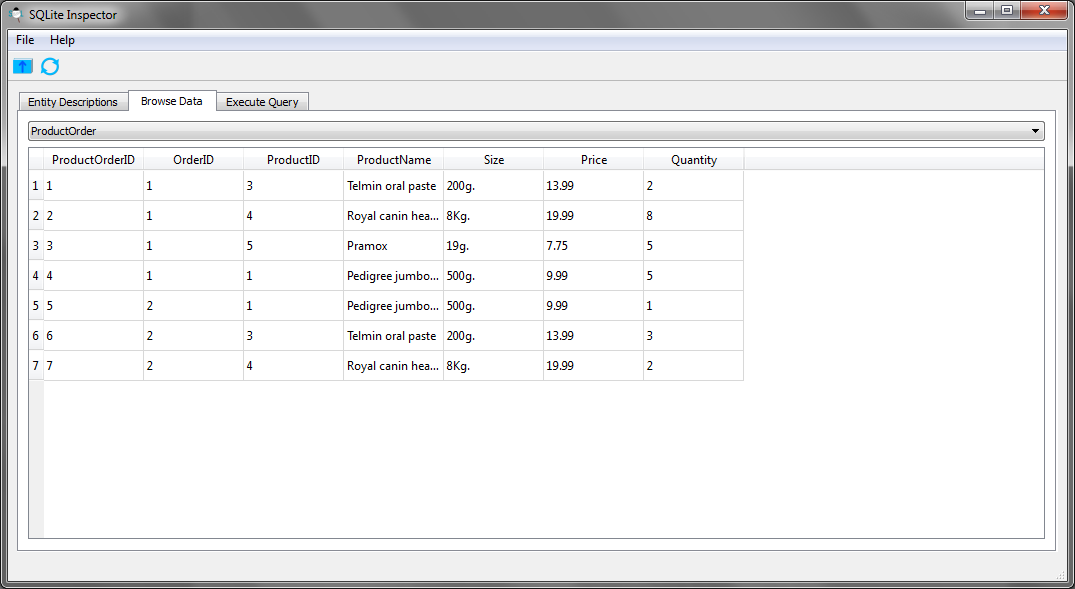
\includegraphics[width=\textwidth]{./TableView4.png}
    \caption{New Entity Relationship Diagram} \label{fig:table-view-4}
\end{figure}

\begin{figure}[H]
    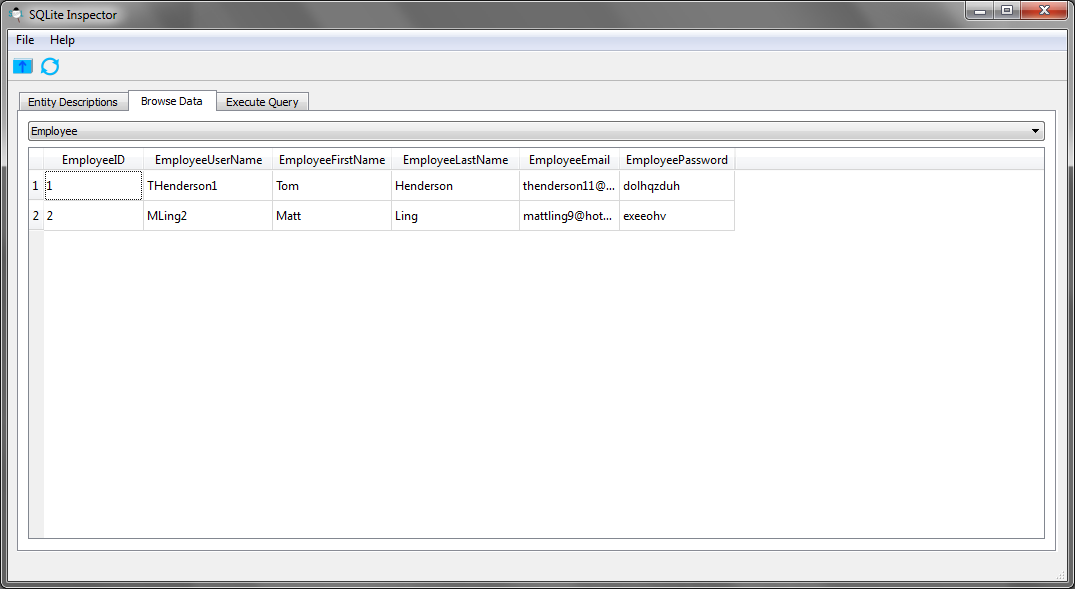
\includegraphics[width=\textwidth]{./TableView5.png}
    \caption{New Entity Relationship Diagram} \label{fig:table-view-5}
\end{figure}

\begin{figure}[H]
    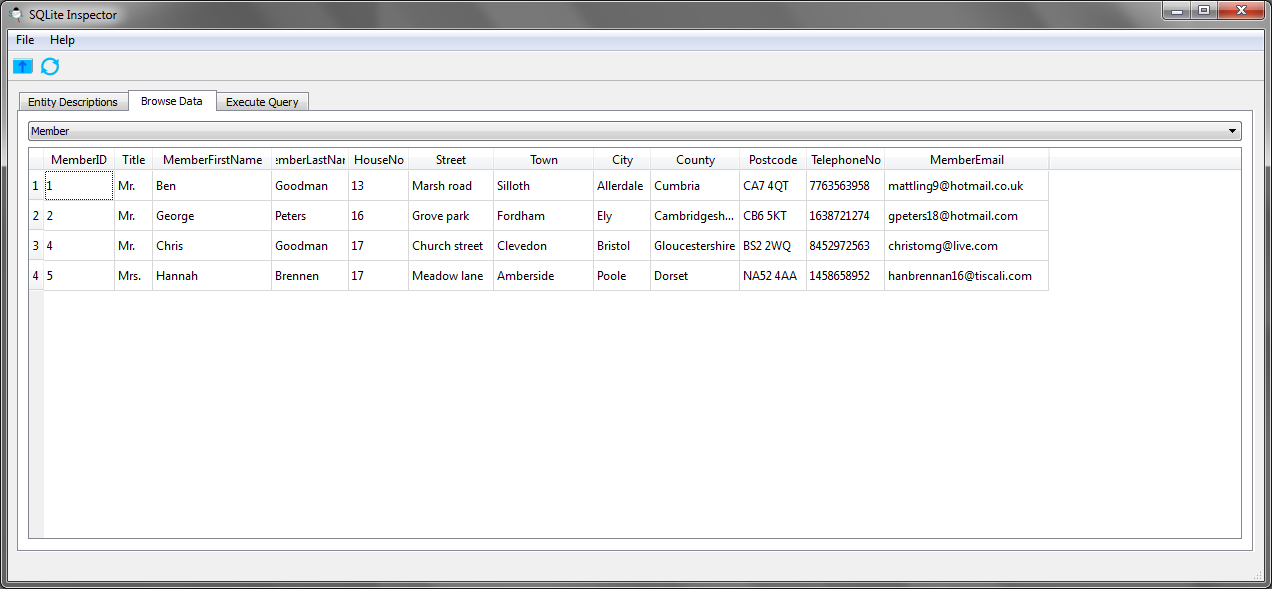
\includegraphics[width=\textwidth]{./TableView6.png}
    \caption{New Entity Relationship Diagram} \label{fig:table-view-6}
\end{figure}

\begin{figure}[H]
    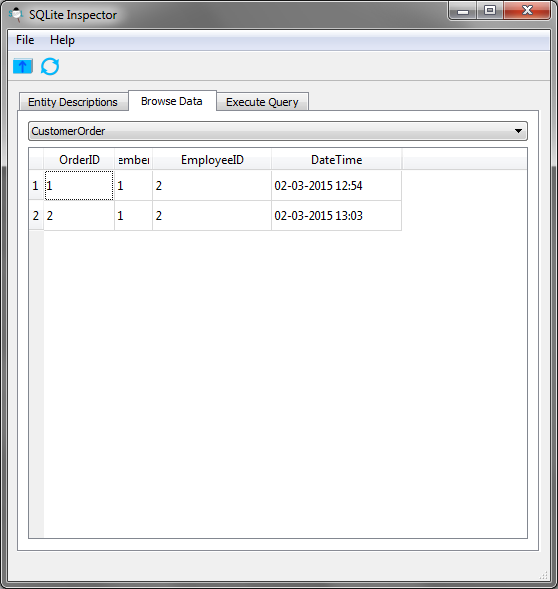
\includegraphics[width=\textwidth]{./TableView7.png}
    \caption{New Entity Relationship Diagram} \label{fig:table-view-7}
\end{figure}

\begin{figure}[H]
    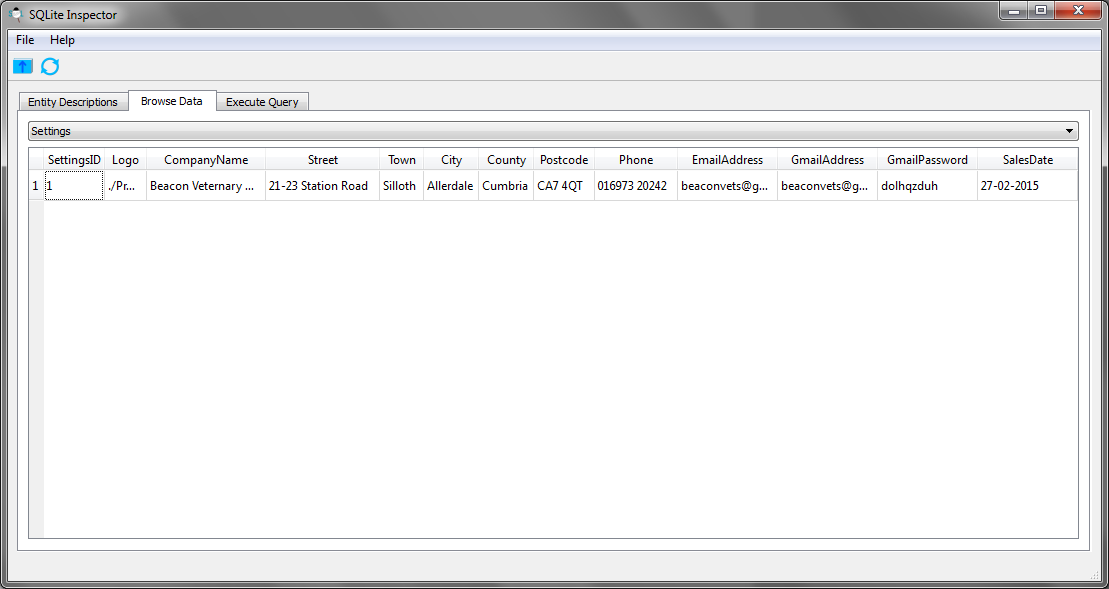
\includegraphics[width=\textwidth]{./TableView8.png}
    \caption{New Entity Relationship Diagram} \label{fig:table-view-8}
\end{figure}


\subsection{Database SQL}

\begin{figure}[H]
	 \caption{SQL for Creating the Product Table} \label{fig:product-sql}
	\begin{sql}
	create table Product
              (ProductID integer,
              ProductName string,
              Size string,
              Price string,
              Category string,
              Location1 integer,
              Location2 integer,
              ImagePath string,
              WeeklySales integer,
              DailySales integer,
              Primary Key(ProductID))
	\end{sql}
\end{figure}

\begin{figure}[H]
	 \caption{SQL for Creating the Weekly Sales Table} \label{fig:weekly-sql}
	\begin{sql}
	create table WeeklyProductSales
          (ProductID integer,
          Date string,
          Sales string,
          foreign key(ProductID) references Product(ProductID))
	\end{sql}
\end{figure}

\begin{figure}[H]
	 \caption{SQL for Creating the Daily Sales Table} \label{fig:daily-sql}
	\begin{sql}
	create table DailyProductSales
          (ProductID integer,
          Date string,
          Sales string,
          foreign key(ProductID) references Product(ProductID))
	\end{sql}
\end{figure}

\begin{figure}[H]
	 \caption{SQL for the Employee Table} \label{fig:employee-sql}
	\begin{sql}
	create table Employee
              (EmployeeID integer,
              EmployeeUserName text,
              EmployeeFirstName text,
              EmployeeLastName text,
              EmployeeEmail text,
              EmployeePassword text,
              Primary Key(EmployeeID))
	\end{sql}
\end{figure}

\begin{figure}[H]
	 \caption{SQL for the Member Table} \label{fig:member-sql}
	\begin{sql}
	create table Member
              (MemberID integer,
              Title string,
              MemberFirstName text,
              MemberLastName text,
              HouseNo integer,
              Street text,
              Town text,
              City text,
              County text,
              Postcode text,
              TelephoneNo integer,
              MemberEmail text,
              Primary Key(MemberID))
	\end{sql}
\end{figure}

\begin{figure}[H]
	 \caption{SQL for the Order Table} \label{fig:order-sql}
	\begin{sql}
	create table CustomerOrder
            (OrderID integer,
            MemberID integer,
            EmployeeID integer,
            DateTime text,
            Primary Key(OrderID),
            foreign key(MemberID) references Member(MemberID),
            foreign key(EmployeeID) references Employee(EmployeeID))
	\end{sql}
\end{figure}

\begin{figure}[H]
	 \caption{SQL for the ProductOrder Table} \label{fig:product-order-sql}
	\begin{sql}
	create table ProductOrder
            (ProductOrderID integer,
            OrderID integer,
            ProductID integer,
            ProductName string,
            Size integer,
            Price integer,
            Quantity integer,
            Primary Key(ProductOrderID),
            foreign key(ProductID) references Product(ProductID),
            foreign key(OrderID) references CustomerOrder(OrderID))
	\end{sql}
\end{figure}

\begin{figure}[H]
	 \caption{SQL for the Settings Table} \label{fig:settings-sql}
	\begin{sql}
	create table Settings
              (SettingsID,
              Logo string,
              CompanyName string,
              Street string,
              Town text,
              City text,
              County integer,
              Postcode text,
              Phone Number text,
              EmailAddress text,
              GmailAddress text,
              GmailPassword text,
              SalesDate text)
	\end{sql}
\end{figure}

\pagebreak
\subsection{SQL Queries}

\begin{figure}[H]
 \caption{SQL for Adding a Product to the database} \label{fig:add-product-sql}
	\begin{sql}
insert into Product (ProductName, Size, Price, Category, Location1, Location2, ImagePath, WeeklySales, DailySales) values(?,?,?,?,?,?,?,?,?)
	\end{sql}
\end{figure}

Figure \ref{fig:add-product-sql} shows the SQL Query used to add a product to the database. The values(?,?,?,?,?,?,?,?,?) are entered by the user as a list. This allows the user to enter different values each time the query is used. This query can be found on page:

\begin{figure}[H]
	 \caption{SQL for Editing a Product} \label{fig:edit-product-sql}
\begin{sql} 
UPDATE Product SET ProductName= ?,  Size = ?,  Price = ?, Category= ?, ImagePath= ? WHERE ProductID = ?
 \end{sql}
\end{figure}
Figure \ref{fig:edit-product-sql} shows the SQL Query used to edit a product in the database. The query only removes the data related to the product associated this query can be found on page: This query can be found on page: 

\begin{figure}[H]
	 \caption{SQL for Editing the stock of a product} \label{fig:stock-sql}
\begin{sql} 
UPDATE Product SET Location1 = ?, Location2 = ? WHERE ProductID = ? 
\end{sql}
\end{figure}
Figure \ref{fig:stock-sql} shows the query used to edit the stock of a product. The stock that is changed depends on the ProductID entered by the user. This query can be found on page: 

\begin{figure}[H]
	 \caption{SQL for Deleting a Product from the database} \label{fig:delete-product-sql}
\begin{sql} 
delete from Product where ProductID = ?
\end{sql}
\end{figure}
Figure \ref{fig:delete-product-sql} Shows the SQL query used to deleted a product form the database. The user enters the ProductID and the query will remove that product from the system. This query can be found on page: 

\begin{figure}[H]
	 \caption{SQL for Adding a Member to the database} \label{fig:add-member-sql}
\begin{sql} 
insert into Member (Title, MemberFirstName, MemberLastName, HouseNo, Street, Town, City, County, Postcode, TelephoneNo, MemberEmail) values(?,?,?,?,?,?,?,?,?,?,?)
 \end{sql}
\end{figure}
Figure \ref{fig:add-member-sql} This query adds a new member to the database.The values entered by the user are entered as a list which means that data must be entered into every field otherwise the sql statement will not work. This query can be found on page:

\begin{figure}[H]
	 \caption{SQL for Editing a Member.} \label{fig:edit-member-sql}
\begin{sql} 
UPDATE Member SET Title = ?,
                                   MemberFirstName = ?,
                                   MemberLastName = ?,
                                   HouseNo = ?,
                                   Street = ?,
                                   Town = ?,
                                   City = ?,
                                   County = ?,
                                   Postcode = ?,
                                   TelephoneNo = ?,
                                   MemberEmail = ?
                                   WHERE MemberID = ?
\end{sql}
\end{figure}
Figure \ref{fig:edit-member-sql} This query edits a member in the database, in order for the query to work the user must provide the new information they want to store along with the product id of the member they want to change.  This query can be found on page: 


\begin{figure}[H]
	 \caption{SQL for Deleting a Member} \label{fig:delete-member-sql}
\begin{sql}
delete from Member where MemberID = ?
\end{sql}
\end{figure}
Figure \ref{fig:delete-member-sql} This query removes a member from the database. the user enters the MemberID, and the query removes that member from the database. This query can be found on page:


\begin{figure}[H]
	 \caption{SQL for Adding an Employee} \label{fig:add-employee-sql}
\begin{sql}
insert into Employee (EmployeeUserName, EmployeeFirstName, EmployeeLastName, EmployeeEmail, EmployeePassword) values(?,?,?,?,?) 
\end{sql}
\end{figure}
Figure \ref{fig:add-employee-sql} This query adds an employee to the database. The relevant data is entered into the query and the query adds it to the Employee table. This query can be found on page:

\begin{figure}[H]
	 \caption{SQL for Editing an Employee} \label{fig:edit-employee-sql}
\begin{sql}
Update Employee SET EmployeeUserName = ?,
                                     EmployeeFirstName = ?,
                                     EmployeeLastName = ?,
                                     EmployeeEmail = ?
                                     WHERE EmployeeID= ?
                                     \end{sql}
\end{figure}
Figure \ref{fig:edit-employee-sql} This query edits the data of an employee. The user enters a EmployeeID and the new information adn the query changes the employee entered by the user. This query can be found on page: 

\begin{figure}[H]
	 \caption{SQL for Deleting an Employee} \label{fig:delete-employee-sql}
\begin{sql}
 delete from Employee where EmployeeID = ?
  \end{sql}
\end{figure}

Figure \ref{fig:delete-employee-sql} This query removes the employee where the user enters the EmployeeID, and the query removes that Employee from the database. This query can be found on page: 

\pagebreak 

\section{Testing}

\subsection{Summary of Results}

My testing proved my system to be very robust and quite reliable, as almost all the results of the tests were as expected (Please go to page \pageref{fig:actual-results} to all the results from the testing)

I found that the main weakness of the testing is that i was not able to test every component of my system. This means there may be problems in my system that my client encounters which i did not. Although i am confident with the robustness of my system, some problems may cause the system to crash however, i am confident that this will not happen as i have tested all the components that could cause the system to crash and all of them worked as expected.

The strengths of my testing was the flow of control between the interfaces. The test proved the user will be able to easily access each interface using the menu bar without any problems occurring. Another strength of my testing was the rigorous testing of the data inputs. I decided that this was the most important area to test as this was where the most problems to occur. Undergoing testing allowed to to identify problems within my system, the problems found during the testing phase have been specified below.

\subsection{Known Issues}

\textbf{Testing the valid characters accepted into the Product Name field.}

In Test series 2.01 i tested to see which characters were eligible for Product Name. Realistically only Letters should be accepted not numbers or special characters. The evidence for this test can be found on page \pageref{fig:test-201-1} figure \ref{fig:test-201-1}, page \pageref{fig:test-201-2} figure \ref{fig:test-201-2} and  page \pageref{fig:test-201-3} figure \ref{fig:test-201-3}. To fix this problem i simply need to amend the regular expression, so that it only allows letters. 



\textbf{Testing the available file types allowed in the Product Image field.}

In test series 2.02, any file type is accepted by the system. However, unless the file is an image file an image will not be displayed. If the user chooses a file which is not an image file, no message is displayed and the system doesn't display an image. The changes that need to be made in order for this test to work, is that if the file is not an image file, do not try to change the current image and display a message to the user saying they need to choose an image file. The system could also restrict the user from choosing and other file than an image file. This could be implemented in a future version of my system.

\textbf{Testing the valid charatcers accepted in the price field.}

In Test Series 2.03, I tested to see the boundaries for a valid price. The evidence from this test series can be found on  page \pageref{fig:test-203-1} figure \ref{fig:test-203-1}, page \pageref{fig:test-203-2} figure \ref{fig:test-203-2}, page \pageref{fig:test-203-3} figure \ref{fig:test-203-3} and page \pageref{fig:test-203-4} figure \ref{fig:test-203-4}. Realistically this should have been between £0.00 and £999.99. However during the Implementation stage i did not set a boundary to the price. Because of this i was able to enter a huge price which should not be allowed. To solve this i need to simply put an if statement every time the user changes the text. To do this I can say: QLineEdit.textChanged.connect(self.check-length). Now to make sure the price is between the limits i need to add: IF self.price < 999.99 THEN: to the self.check-length method. if the price is less than 999.99 then i need to change the QLineEdit boarder to green. This can be done by applying a style-sheet to that specific QLineEdit.

Also, the user can enter a price into the price field. I used a built in validator that only allows integers from the keyboard to be entered. However this module allows the use of an exponential to be entered, which allows the user to enter the letter 'e'. This means that this test failed as it should only accept integers. To change this, i need to tell the validator which notation to use. At the moment it uses both standard and scientific notation. The scientific notation is what allows the user to enter the letter 'e'. To stop this from happening i need to set the notation to just the standard notation. This can be done easily by simply doing self.price-validator.standardNotation() where self.price-validator is a QDoubleValidator.

\textbf{Testing to see which characters are available in the Member Name field}

In test series 2.05, the only acceptable characters in the members name should be letters. special characters or numbers should not be accepted. At the moment, special characters are not accepted however letters and numbers are. This has been evidenced on page \pageref{fig:test-205-1} figure: \ref{fig:test-205-1}  and page \pageref{fig:test-205-2} figure: \ref{fig:test-205-2}. To change this, i need to change the regular expression so that integers should not be accepted. The regular should look along the lines of this: "[A-Z]{1,18}" where the A-Z is the range  of acceptable characters and 1-18 is the amount of characters allowed. 


\textbf{Testing the functionality of the find postcode button}

When the member enters their postcode, They have the ability to search for their address if they live im Cumbria. However, the postcodes stored in the CSV file have spaces in. The postcode field still validates the postcode even if there is no space in it. Therefore the user could enter their postcode and because it does not have a space in it, it won't be found. for example if 'CB7 5LQ' was stored in the CSV file and the user entered 'CB75LQ' it would not be found. To solve this problem i should change all of the postcodes in the CSV so they do not have spaces in. Then when the user enters their postcode, remove the space if there is one. This can be done by doing 'postcode-input.replace(" ",""). This would now allow the user to either enter the postcode with or without a space and it will still be able to be found in the CSV file.

\textbf{Testing the valid characters allowed in the house number field}

In this test, i tested the range of characters that were acceptable for the house number. Originally i thought that only integers should be accepted in this field. Since the implementation stage, i have realised that houses can also contain letters as well. for example there could be a 66A or a 66B or the house could have a house name instead of a number which the user could not specify in my current system. Therefore,  this test has failed. To improve this feature, i should change the the input method so that the user can also enter characters in the field as well.

\textbf{Ensuring all data is stored in the Member table in the correct format.}

 Ideally i want every postcode to be stored without a space between them. Currently the user can choose to enter a space or not which will mean that some will be stored with a space between and some will not. This issue will be resolved if the changes to test series 2.09 are made.

\textbf{Right Clicking on an employee when not signed in on the administrators account}

in this test, the menu that is displayed when the user right clicks on an Employee in the search window. When logged in on an account that is not the Administrators, the user should not be able to access the Add Edit And Delete Employee. However, when the user right clicks on an Employee they are given the option to edit or delete an Employee. This should not happen, instead i want these options to be greyed out if the user is not signed in as the administrator. To do this, when the user right clicks on one of the Employees, a function is run to display the menu to the user. To solve this problem, i need to check whether the user is signed in as the administrator and then choose whether to display the edit and delete Employee options or grey them out. I already have a function that returns the EmployeeID of the currently logged in user, i can use this to check who is currently logged in. I can then use an if statement stating: IF EmployeeID != 1 THEN. Now i need to say what must happen if they are not signed in on the administrators account, in this case i want to grey out the menu options, which can be done by doing: QMenuItem.setDisabled(True)
\pagebreak

\section{Code Explanations}

\subsection{Difficult Sections}

\subsubsection{Creating the Custom TitleBar} 

The figure below shows line 1 to 32 from the CustomToolbarClass.py file. The full file can be found on page \pageref{fig:CustomToolbarClass}.

\pythonfile[firstline=1, lastline=32]{./Maintenance/CustomToolbarClass.py}

After learning how to make the titlebar, i learnt that the titlebar was just a widget. The titlebar widget contains a QLabel, and two QToolbuttons.

\pythonfile[firstline=10, lastline=19]{./Maintenance/CustomToolbarClass.py}

Here the close and minimise buttons are being created. each button is an instance of a QToolButton. 

\begin{python}
self.minimise.setIcon(QIcon(".\SystemImages\minimize.png"))
\end{python}

The line above assigns an image to the tool button. minimize.png is an image i created using Adobe Photoshop CS6.

\pythonfile[firstline=24, lastline=30]{./Maintenance/CustomToolbarClass.py}

The above section of code shows all of the widgets being added to a QHBoxLayout. Spacing and stretching is applied to the widget so that the label is on the other side of the screen to the Toolbuttons. I then added a style sheet to the toolbar so it matched the style of the rest of my system. To see the style sheet for the titlebar, please refer to page \pageref{fig:CustomToolbarClass} in the code listing section. \par

i have provided a diagram below to help improve your understanding of the title bar.



\begin{figure}[H]
    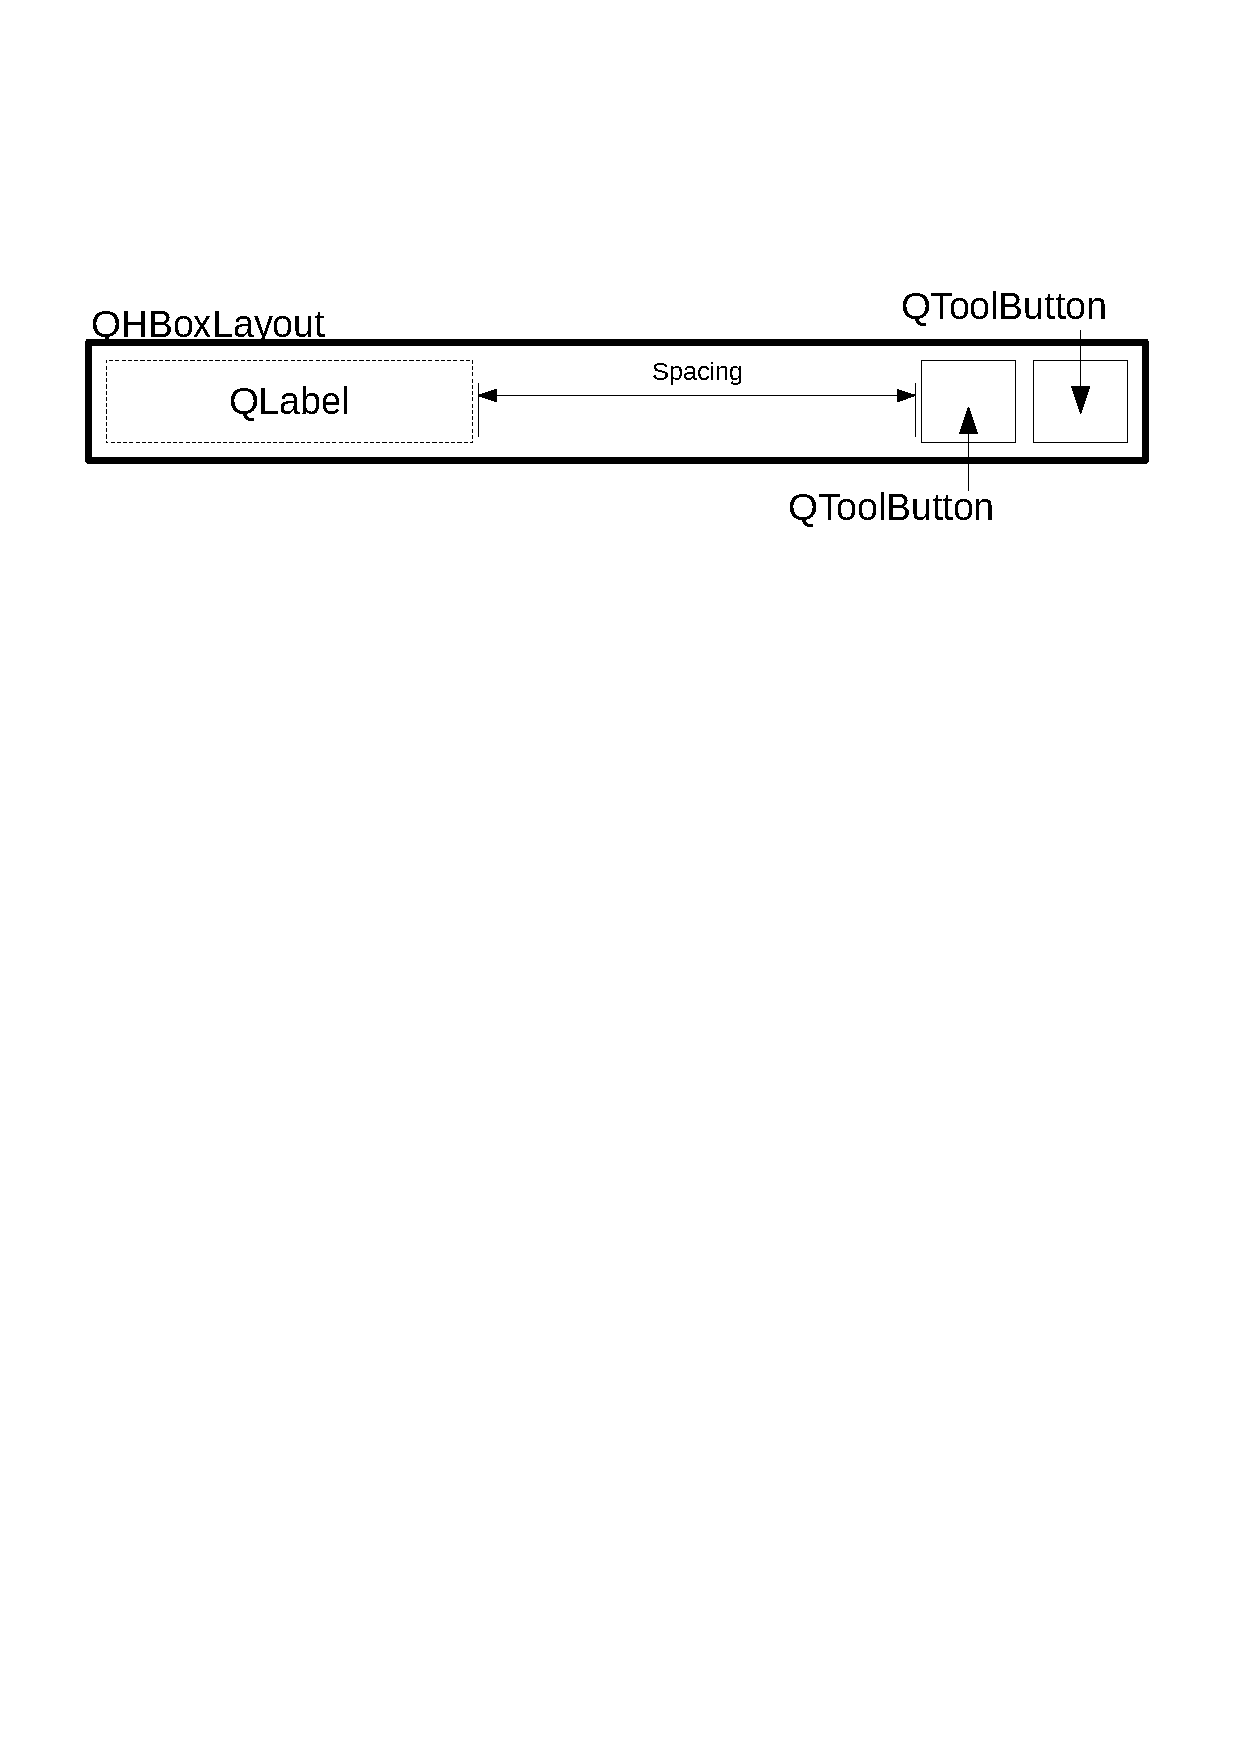
\includegraphics[width=\textwidth]{./titlebar-diagram.pdf}
    \caption{Structure of Titlebar.} \label{fig:titlebar-diagram}
\end{figure}

Finally, to add the widget to the main window, an instance of the CustomTitleBar is created in the main program, and added to a QVBoxLayout. The QVBoxLayout also contains the QMenuBar and the QStackedLayout that allows the user to change between interfaces. The code below shows the default titlebar and window frame being hidden, (Allowing the user to use the titlebar. Methods are attached to the close and minimise buttons to close the window or minimise the window when they are clicked.

\pythonfile[firstline=63, lastline=73]{./Maintenance/CustomToolbarClass.py}

\textbf{Plotting sales on a graph and adding an average line to predict the future sales of the product}

Below i have provided the full code that creates the graph. This code can also be found in the StockManagementClass.py file on page \pageref{fig:StockManagementClass} in the code listing section.

\pythonfile[firstline=123, lastline=184]{./Maintenance/StockManagementClass.py}

having the DailyProductSales and WeeklyProductSales tables in the database allowed me to plot data to the graph easily. When the user wants to display the graph of sales for a specific product they enter the ProductID into the ProductID field. Here the ProductID is searched to see if there has been any sales in the DailyProductSales or WeeklyProductSales tables. If any sales have been made the sales gets returned as a list. the sales made are stored in the `sales' list and the date the sales were made are stored in the `dates' list. This is show below.

\pythonfile[firstline=126, lastline=133]{./Maintenance/StockManagementClass.py}

\pagebreak

\pythonfile[firstline=136, lastline=141]{./Maintenance/StockManagementClass.py}

The code above prepares the x and y values ready to be plotted to the graph.

\begin{python}
if dates:
\end{python}

The code above is used to say that; only add the sales and dates the the x and y values if sales have been made, if no sales have been made, do not assign any values to x and y and do not plot any values.

\pythonfile[firstline=137, lastline=141]{./Maintenance/StockManagementClass.py}

The code above adds the sales dates to the x axis list and adds the amount of sales to the y axis list. The variable `value' puts the date and the sales made on that date together and stores them under a single variable. This variable is then added to a list of all the other dates and sales that are going to be plotted to the graph. this list is named `data'. Next, all the dates in which sales were made are added to the x axis list and all the sales made on that date are added to a y axis list. These lists are then use to plot the data onto the graph. The graph is plotted using the following code:

\pythonfile[firstline=143, lastline=154]{./Maintenance/StockManagementClass.py}

To calculate the future sales of the product i create a line of best fit for the data plotted. The code to create the line of best fit has been supplied below:

\pythonfile[firstline=157, lastline=173]{./Maintenance/StockManagementClass.py}

To predict the stock for the next week, i take the line of best fit from the graph, because the line of best fit is  a straight line, the gradient is constant, therefore the increase in sales between each week will be constant. If i work out the change in sales between each week, and add this to the sales made this week, that will provide me with a prediction for the sales made next week. 

\begin{python}
(m,c) = polyfit(x,y,1)
\end{python}

The gradient and the line of best fit are calculated for me using the polyfit module. I have assigned the gradient to the variable `m' and the y intercept to the variable `c'. I plot the line of best fit using the polyval module. The variable `yp' is assigned to a list of x and y values for the line of best fit. to calculate the change in the Y value each day or each week i simply take the sales made on a specific day and minus the sales made the day before. This will get the change in Y for each value of X. For example if 2 more sales were made each day after 10 days, 20 more sales would have been made. I assign the change in Y value to the variable `difference'. the difference was not always an integer, mostly it was a long decimal number there i rounded the difference to 2 decimal places and assigned this value to a new variable called `rounded-difference'

\begin{python}
yp = polyval([m,c],x)
difference = yp[1] - yp[0]
rounded_difference = round(difference, 2)
\end{python}

Now that i knew the difference between each day or week, i needed to know the last sale made. This was done by finding the length of the y values list and then using the length of the list to get the last item in the list. I assigned the last sale made to the variable `last-sale'.

\begin{python}
length_of_list = len(yp)
last_sale = yp[length_of_list - 1]
#PLEASE NOTE - i used length of list - 1 because list items in python start at 0 not 1.
\end{python}

now that i knew how many sales were last made, i simply need to add the difference between each day to the last sale made, to calculate the sales for next week.

\begin{python}
predicted_sale = last_sale + rounded_difference
rounded_predicted_sale = int(round(predicted_sale, 0))
self.prediction.setText(str(rounded_predicted_sale))
\end{python}

the predicted sale is then rounded, and assigned to the variable `rounded-predicted-sale' this is then set as the text to the stock prediction QLineEdit.

\pagebreak

\subsubsection{Emitting a signal when a QLabel is clicked.}

Unlike a QPushButton, a QLabel does not have a pre-existing .clicked.connect() signal. Therefore i had to create a new QLabel that will emit a signal when it is clicked. The code below is the class i made for the new QLabel.

\begin{python}
class ExtendedQLabel(QLabel):
 
    def __init(self, parent):
        QLabel.__init__(self, parent)
 
    def mouseReleaseEvent(self, ev):
        self.emit(SIGNAL('clicked()'))
\end{python}

in the constructor on line 3, i stated that the class, ExtendedQLabel, is a child/sub class of QLabel which inherits all of its attributes. This was done by passing parent into the constructor. I then included a new method for the ExtendedQLabel on line 6 called "mouseReleaseEvent". Looking at line 6 and 7, this will emitt the clicked() signal once the mouse has been left clicked and released. Now that the ExtendedQLabel emits a signal when it is clicked, i need to attach a method to be run when this signal is emitted. The image below shows the ExtendedQLabel in use:

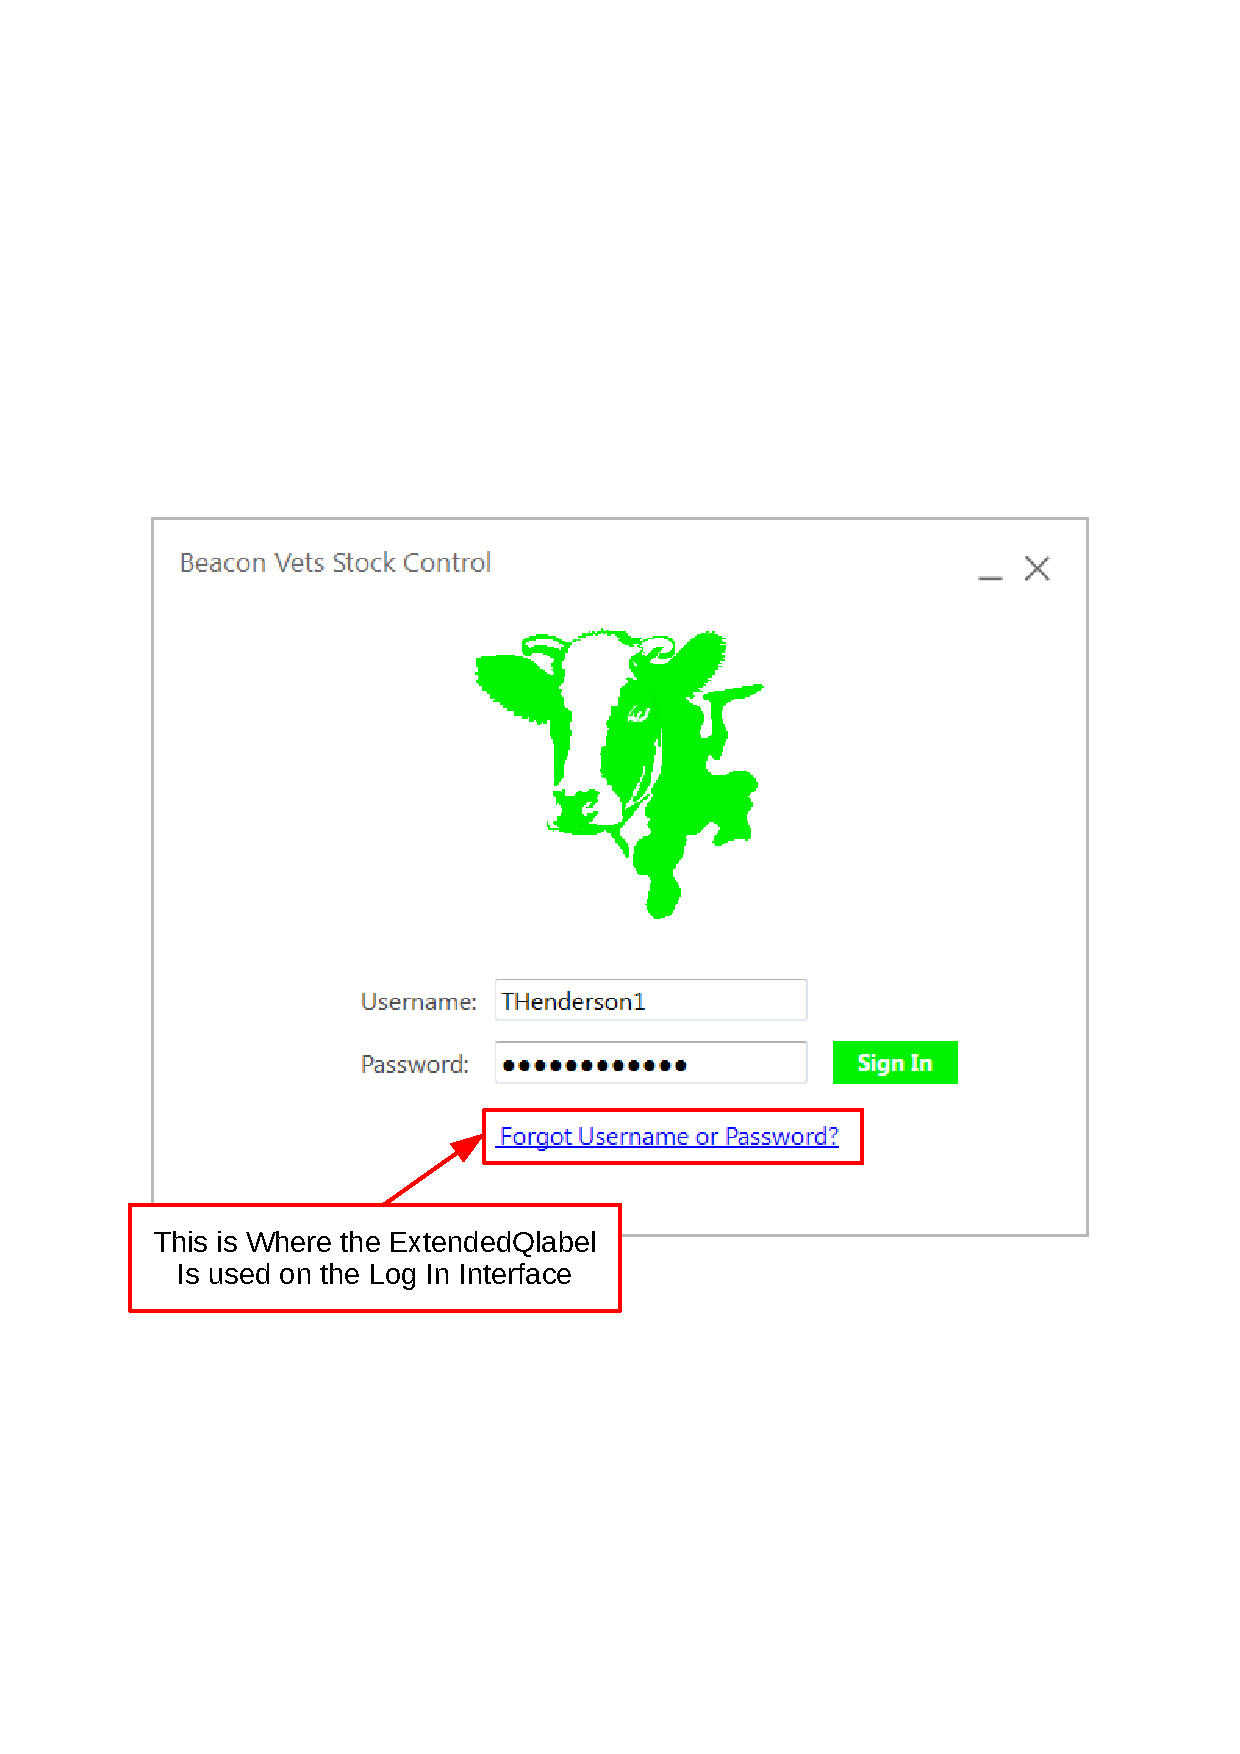
\includegraphics[width=\textwidth]{./ExtendedQLabelImage.pdf}

The code below shows how i connected a method when the clicked() signal is emitted. Line 1 shows how a QPushButton is connected to a method through its built in signal and Line 2 shows how to connect a method when the 'clicked()' signal is emited from the QLabel.

\begin{python}
self.log_in_instance.enter_button.clicked.connect(self.find_account)
self.log_in_instance.connect(self.log_in_instance.forgot_password, SIGNAL('clicked()'), self.reset_password)
\end{python}

In Line 2, "self.log-in-instance.forgot-password" is the variable assigned to the ExtendedQLabel, the SIGNAL('clicked()') is the signal that is emitted when the label is clicked and the self.reset-password is the method that is run when the signal is emitted. The self.reset-password method simply changes the index of the stacked layout to the index of the forgot password interface.

\subsubsection{Adding a right click menu to items in a table.}

To improve the ease of use of the system i wanted the suer to be able to right click on a product and be able to go straight to the edit product interface, delete product interface or manage stock interface directly. This is a far better option than using the search window to find the ProductID of the product, click on the product menu go to the edit product interface, enter the ProductID and click on the find button. I First created the individual menus that will be displayed when the user right clicks either a product member or employee, the code for this is shown below.

\begin{python}

self.search_instance = SearchClass()
        
self.search_instance.product_right_click_menu.addAction("Manage Stock" , self.EditStock)
self.search_instance.product_right_click_menu.addAction("Edit Product" , self.EditProduct)
self.search_instance.product_right_click_menu.addAction("Delete Product" , self.DeleteProduct)

self.search_instance.member_right_click_menu.addAction("Edit Member" , self.EditMember)
self.search_instance.member_right_click_menu.addAction("Delete Member" , self.DeleteMember)

self.search_instance.employee_right_click_menu.addAction("Edit Employee" , self.EditEmployee)
self.search_instance.employee_right_click_menu.addAction("Delete Employee" , self.DeleteEmployee)

These menus were not created inside the SearchClass class because i needed to connect methods that were visible in the main program but were not visible in the SearchClass. Examples of these methods are self.EditProduct and self.EditStock which take the user to the edit product and edit stock interface. Which menu is displayed, depends on which table is currently being displayed. For example if the user is currently finding a Member in the Member table, when they right click on one of the Members i want member-right-click-menu to be displayed not the one for the product or the employee. To record which table is currently being viewed i simply took the current index of the combo box, in which the user chooses which table they want to display.The following code decides which right click menu to use depending on the current index of the combo box.

\begin{python}
 if self.table_combo_box.currentIndex() == 0:
	 self.product_right_click_menu.exec_(self.mapToGlobal(position))
 elif self.table_combo_box.currentIndex() == 1:
	self.member_right_click_menu.exec_(self.mapToGlobal(position))
elif self.table_combo_box.currentIndex() == 2:
	self.employee_right_click_menu.exec_(self.mapToGlobal(position))
\end{python}

Lines 2,4 and 6 will display the appropriate menu when right clicked by the user. When the user right clicks, for example, on a product in the Finding Product table, and clicks on edit rpoduct from the drop down menu, the user is taken automatically to the edit product interface with the ProductID already entered and found. To retrieve the ProductID from the item in which the user has clicked on is shown below.

\begin{python}
self.indexes = self.display_table.selectionModel().selection().indexes()
rows = []
for selected_row in self.indexes:
	row_number = selected_row.row()
	if row_number not in rows:
		rows.append(row_number)      
no_of_rows_selected = len(rows)
if no_of_rows_selected == 1:
            #gets the product_id of product selected
            self.product_id = self.model.record(rows[0]).field(0).value()
\end{python}

'self.indexes' is a list that stores the index of the row and column that the user selects. For example if the user selects rows 3 column 4 and row 5column 6 at the same time, 'self.indexes = [(3,4),(5,6)]' Usually the user will only select one row, which will mean self.indexes will only contain one index. The row of the selected index is extracted using 'selected-row.row()' on line 4 in the code above. each row is selected is then added to a list called 'rows' on line 6. To get the Product, Member or Employee ID of the row selected, only one row must be selected otherwise an error occurs. to prevent the error from occurring, i just included an IF statement saying if 'len(rows) != 1' where rows is a list of the currently selected rows. This can be found on line 8 where i have just assigned a variable to the length of the list 'rows'. If the length of the list does equal one, then the system gets the ID from the table on line 10 and assigns it to the variable 'self.product-id'. This ID is then used to if the user does decide to edit the product for example, because it is automatically entered by the system.


\pagebreak

\subsection{Self-created Algorithms}

\subsubsection{Calculating New Quantity}

The following algorithm calculates how many of a specific product are currently in the order updates the quantity accordingly. For example if there are currently 5 in the order, adding another product will change the quantity to 6.

\pythonfile[firstline=448, lastline=467]{./Maintenance/CreatingOrderClass.py}

\begin{python}
if product_info[0][0] == int(self.current_order.item(row,0).text()):
\end{python}

the line above checks to see whether the product in which the user has clicked on is already in the current order table or not.

\begin{python}
new_quantity = int(self.current_order.item(row,4).text()) + 1
self.current_order.setItem(row,4, (QTableWidgetItem(str(new_quantity))))
inTable  = True
\end{python}

the code above is only run if the product is already in the current order table. This takes the current quantity of the product and increases it by one. this is assigned to the variable `new-quantity'. this new quantity is then changed in the quantity field in the current order table. Then the system is told that the product is currently in the table.

If the product is already in the table and once the quantity has been updated the total price for the products = (price of product * quantity) this is done in the code below:

\begin{python}
if inTable == False:
            new_row = (self.current_order.rowCount())
            self.current_order.insertRow(new_row)
            count = 0
            for item in product_info[0]:
                self.current_order.setItem(new_row, count, (QTableWidgetItem(str(item))))
                count += 1
            self.current_order.setItem(new_row, 4, (QTableWidgetItem(str(1))))

        self.price = 0.00
        for row in range(0, self.current_order.rowCount()):
            self.price += float(self.current_order.item(row,3).text()) * float(self.current_order.item(row,4).text())
\end{python}

\pagebreak

\subsubsection{Calculating Whether a product needs to be restocked.}

The following algorithm, takes the current stock of a product and calculates whether the product need to be restocked.

\pythonfile[firstline=575, lastline=610]{./Maintenance/AddingRemovingData.py}

\begin{python}
restock_list = []
move_list = []
\end{python}

The following code is very simple, it creates the list of all the products that need to be restocked and the list for the products that require stock to be moved form one location to the other. Eventually, the restock-list will contain the ProductID of all the products that need to be restocked and move-list will contain the ProductID of all the products that need to have stock moved form one location to another.


\begin{python}
product_cursor = db.cursor()
product_cursor.execute( "Select ProductName from Product WHERE 1=1")
product_id_list = product_cursor.fetchall()
\end{python}

The code above creates a cursor to execute the SQL query. The SQL query simply selects every ProductName in the Product table. Each Product Name is then added to a list named product-id-list. 

\begin{python}
for item in product_id_list:
            stock_cursor = db.cursor()
            sql = "Select Location1, Location2 from Product WHERE ProductName = ?"
            stock_cursor.execute(sql, (item))
            stock_list = stock_cursor.fetchall()
            total_stock = int(stock_list[0][0]) + int(stock_list[0][1])
            if total_stock < 5:
                restock_list.append(item)
            if int(stock_list[0][0]) < 5:
                move_list.append(item)
\end{python}

The code above is run for each product in the database. This is done by line 1 in the code section above. The stock in Location1 and the stock in Location2 are retrieved from the database using the SQL query in line 3. The variable ``total-stock'' is assigned to the product of the stock in each location. If the total stock of the product is less than 5, then the product name of that specific product is added to the restock list because the client will need to buy more stock if there are 5 or less left in total. Line 9 and line 10 add the Product Name of the current product to the move-list if the stock in Location1 is less than 5. If the stock in Location1(the Shop) is less than 5 then stock needs to be moved from Location2(The storage room) to the shop.

Once the the algorithm has checked every product in the database and has populated the two lists with the product names of the products that need to be restocked and stock that needs to be moved between locations, this information needs to be displayed to the user.

\begin{python}
if restock_list:
            message = "Warning! \n \n The following products need to be restocked: \n \n "
            for product_name in restock_list:
                message += "-{0} \n".format(product_name[0])
            self.error_message_instance = ErrorMessageClass(message)
            self.error_message_instance.move(750,400)
            self.error_message_instance.show()
            self.error_message_instance.raise_()
\end{python}

Line 1 in the code above will only run the following code if there are actually any products in the restock-list. If there are no products that need to be restocked, then there is no need to run the code above. This will prevent my system running any code unnecessarily. The variable ``message'' will eventually be a string that will tell the user that products need to be restocked and will then list all of the products below. the string message is then inserted into an instance of an Error Message. An Error Message is simply a pop up window, with a QLabel that displays a message to the user and an `Ok' button so the user can tell the system they have read the message.The string `message' is the text that shall be displayed in the QLabel. The image below gives a better understanding of the window that is displayed.

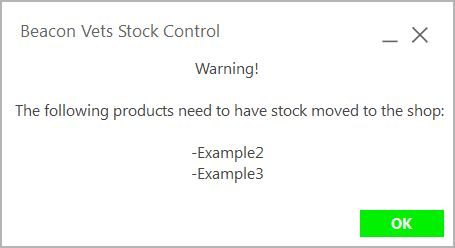
\includegraphics[width=\textwidth]{./error.jpg}
\label{fig:move-stock-message}

\begin{python}
elif move_list:
            message = "Warning! \n \n The following products need to have stock moved to the shop: \n \n"
            for product_name in move_list:
                message += "-{0} \n".format(product_name[0])
            self.error_message_instance = ErrorMessageClass(message)
            self.error_message_instance.move(750,400)
            self.error_message_instance.show()
            self.error_message_instance.raise_()
\end{python}

The code above is very similar to the previous code however, this will create an Error message that tells the user which products need to be moved from one location to another. The string message is created saying: ``Warning! The following products need to have stock moved to the shop:''. Then every ProductName in the move-list is added to the string. This string is then used on a QLabel in a Error Message Instance.

\pagebreak

\subsubsection{Sending a 4 digit code to an email address.}

As a security measure, if an employee is logged in and they want to change their password, they must enter a 4 digit code sent to their email address. This is so that if they are logged in to the system, someone cannot come along and simply change the employees password. The code below generates the code and sends it to the users email address. It can also be found on line 820 in the Main Program section of the Code Listing on page \pageref{X}

\begin{python}
def send_code_to_email(self, username):
        settings = getSettings()
        self.code = random.randint(1000,9999)
        decrypted_password = change_password(settings[0][11], -3)
        employee_info = find_employee_by_username(username)
        message = "Hello {0}, \n \n Your Reset Password Code is:  ".format(employee_info[0])
        msg = "\r\n".join([
          "From: beaconvets@gmail.com",
          "To: {0}".format(employee_info[2]),
          "Subject: Password Reset Code",
          "",
          ("{0}{1}".format(message ,str(self.code)))])
        mail = smtplib.SMTP('smtp.gmail.com','587')
        mail.ehlo()
        mail.starttls()
        mail.login('{0}'.format(settings[0][10]) , decrypted_password)
        mail.sendmail('{0}'.format(settings[0][10]), str(employee_info[2]) , msg)
        mail.close()
\end{python}

The actual 4 digit code is generated on line 3. I used the random function in python to generate the number. Because the code needed to be four digits, I set the range of the random number between 1000 and 9999. Line 4 decrypts the password used to send the emails so the system can log into the email account and send the code from the email address. 

The variable 'message' is assigned to a string that will represent the contents of the email. The string will be greet the user and will give them the four digit. I used an SQL query to take the EmployeeFirstName associated with the account, so that the email will say "Hello John, your password reset code is ..... or Hello Sarah, your password reset code is ......". Lines 8-10 tell will say the email address the email was sent from, the subject of the email, and the email address the email was sent to. In this case, the To: section is assigned to the employee email address stored within the system. Lines 13-18 logs into the email account and sends the email to the email address.

\pagebreak

\subsubsection{Entering data from a CSV file.}
When the user searches for their postcode using the find button on the Add Member interface, if the postcode is in the CumbriaPostcodes.csv file, the system takes the county and town from the CSV file and enters the data into the data fields of the system. The screenshot below shows the user entering a postcode from the CSV file into the postcode field, before they click the find button.

\begin{figure}[H]
\caption{Screenshot before the user clicks the find button.} \label{fig:find-postcode}
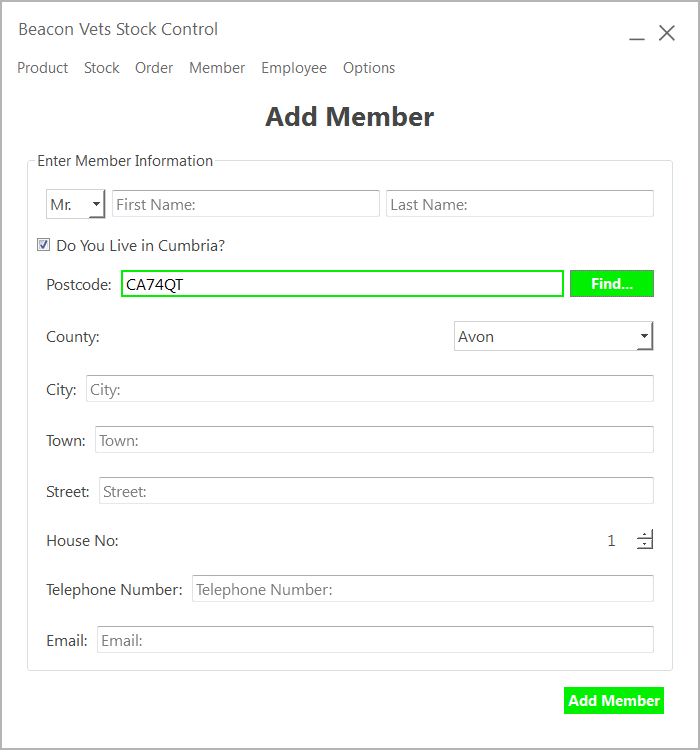
\includegraphics[width=\textwidth]{./208-2.png}
\end{figure}

The screenshot below then shows the result from the user clicking the find button. you can see that the County and Town fields have automatically been changed by the system.

\begin{figure}[H]
\caption{Screenshot after the user clicks the find button.} \label{fig:found-postcode}
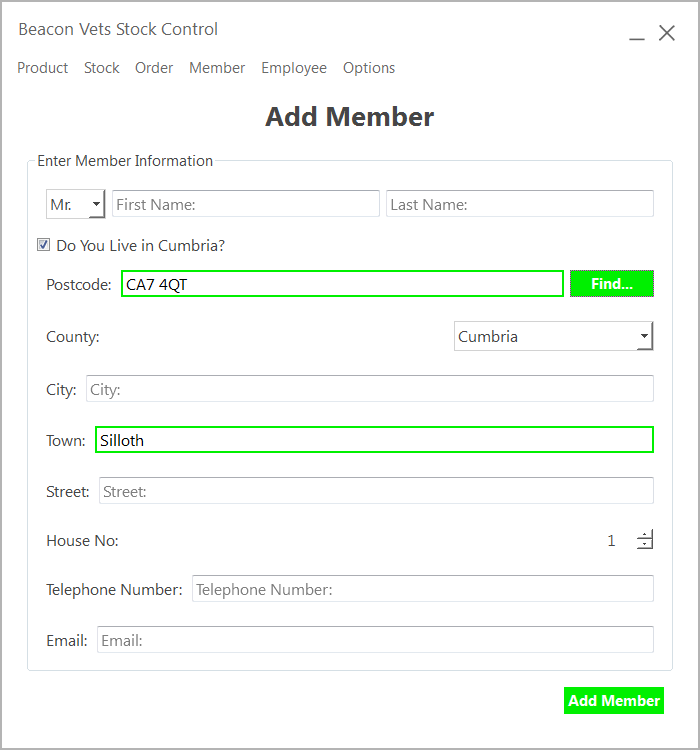
\includegraphics[width=\textwidth]{./208-1.png}
\end{figure}

In order to manipulate the data from the CSV file it needed to be changed so that python can use the data. The following code, opens the CSV file, and adds each address to the list 'self.county-list" . Now the data is in a list, python can use the data from the CSV file. 

When the 'Find' button is clicked in figure \ref{fig:find-postcode}, the system searches to see if the postcode matches any of the postcode in the address list. Each address is a list containing the postcode, the county then the town. To code below shows how i searched for the postcode.

\begin{python}
self.postcode_input = self.postcode.text()
self.postcode_input = self.postcode_input.upper()
for count in range(0, len(self.address_list)):
	if self.postcode_input in self.address_list[count]:
\end{python}

self.postcode-input is assigned to the postcode entered into the postcode QLineEdit. this is done using self.postcode-input = QLineEdit.text(). Line 2 simply changes the postcode into all upper case before it is searched for. A FOR loop is then run for each item in the postcode list, and an IF statement is used to match the postcode entered by the user and the postcode stored under each address. If the postcode does not match the system will move onto the next address until it has been searched under every address in the list. If the postcode entered by the use does match the postcode stored in one of the addresses then The following code is run.

\begin{python}
self.postcode.setText(self.address_list[count][0])
self.index = self.county.findText(self.address_list[count][2])
self.county.setCurrentIndex(self.index)
self.town.setText(self.address_list[count][1])
self.validate_town
\end{python}

The town was easy to change as the town data field is a QLineEdit. Entering a string into this field is easy, using QLineEdit.setText(string). The town was set on Line 4 in the code sample above, where self.address-list[count][1] is the town of the matching address. Changing the County prooved to be more difficult because the data field was a QComboBox not a QLineEdit. A QComboBox requires the user to select an option from the list provided and does not support the ".setText" feature. Instead, the QComboBox has to be searched for the County from the CSV file. if the county is in the file the '.findText' method will return the index of the county in the QComboBox. 'QComboBox.setCurrentIndex(index)' can then be used to change the index to the index of the county that matches the address. This was done on lines 2 and 3 from the code snippet above.

\subsubsection{Populating a QComboBox from a text file.}

When adding a Member to the system the user needs to enter the County in which the Member lives. I used a QComboBox for the counties as using a QComboBox does not require the field to be validated. I know that hard coding all of the postcodes into the system would be a very long and tedious process so i decided to use a text file containing the counties and used this to populate the Combo box.

The code below opens the text file named 'Counties.txt' and adds each county from the file into the list 'self.county-list'.

\begin{python}
with open("Counties.txt",mode="r",encoding="utf-8") as myFile:
                    for line in myFile:
                        self.county_list.append(line.rstrip("\n"))
\end{python}

Now that self.county-list is populated with each county, i can use this list to populate the combo box.

\begin{python}
for item in self.county_list:
                        self.county.addItem(item)
\end{python}

The code above adds each county in the self.county-list to the ComboBox. This is done using a FOR loop for each item in the list. The item is added to the combo box using QComboBox.addItem(county)

This method off adding the counties to the QComboBox was far simplier and far more code efficient than other methods.

\pagebreak

\subsubsection{Preventing users from being able to click the add, edit and delete member if they are not signed in on the administratory account.}

I had to prevent users from ebing able to add edit or delete employees if they are not logged in on the administraor account. In order to check this, i decided to check the EmployeeID of the currently logged in use. If the EmployeeID is 1 then the user is logged in on the administrator account, otherwise they are not. This is checked, once the Employee's Log in details have been verified upon log in, but before they are presented with the creating order interface. To get the EmployeeID, i used an SQL statement to return the EmployeeID where the EmployeeUsername is the Username entered by the user. The code below is only run if the user has successfully logged in.

\begin{python}
self.menu.show()
username = find_employee_by_username(self.log_in_instance.username.text())
EmployeeID = username[3]
if int(EmployeeID) != 1:
	self.add_an_employee_action.setDisabled(True)
	self.edit_employee_action.setDisabled(True)
	self.remove_an_employee_action.setDisabled(True)
	self.explanation_action.setVisible(True)
else:
	self.add_an_employee_action.setEnabled(True)
	self.edit_employee_action.setEnabled(True)
	self.remove_an_employee_action.setEnabled(True)
	self.explanation_action.setVisible(False)
	check_for_stock_updates(self)

\end{python}


The code above varies the visibility and clcikablility of each option in the Employee menu. Looking at line 4, this runs an IF function as to whether or not the employee currently logged in is an administrator(if their EmployeeID = 1 or not) If the user is currently logged into the Administrator account, then the Add Edit and Delete Employee should be visible and clickable and the Option telling the user why they cannot click the Add Edit and Delete Employee buttons should not be visible. This is done on lines 10 to 14. If the user is not currently logged in the administrators account, then the Add Edit and Delete buttons should be visible but not clickable and the Option telling the user why they cannot click on the add edit and delete employee options should be visible and clickable. This is done on lines 5-8. Figure \ref{fig:admin-employee-menu} shows the Employee menu that is displayed when logged in on the admin account and figure \ref{fig:non-admin-employee-menu} shows the Employee menu that is displayed when the user is not logged in on the admin account.



\begin{figure}[H]
\caption{Employee menu when logged in on the administrator account} \label{fig:admin-employee-menu}
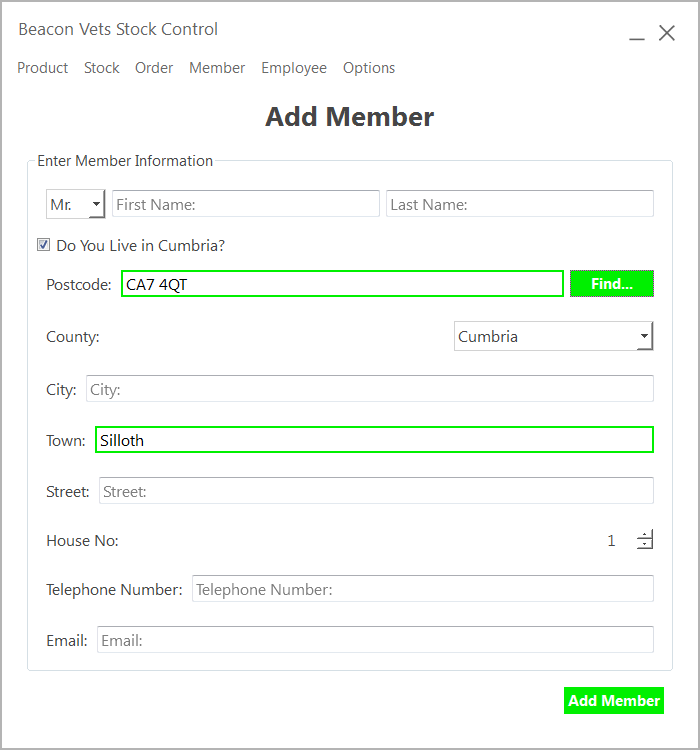
\includegraphics[width=\textwidth]{./208-1.png}
\end{figure}


\begin{figure}[H]
\caption{Employee menu when not logged in on the administrator account} \label{fig:non-admin-employee-menu}
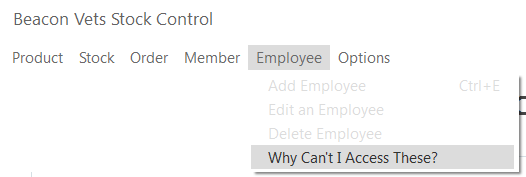
\includegraphics[width=\textwidth]{./non-admin-employee-menu.png}
\end{figure}





\section{Settings}

When managing the stock of the products, the user gets displayed a graph which shows the sales of the product either by week or by day. This graph was implemented into my system using the matplotlib library. The matplotlib library does not come with the installation in python. The easiest way to install matplotlib is by using PIP, a tool that does come with the python installation that installs the library you want, along with all the dependencies it requires to work. To install pip on Windows, the user can type `` python3 get-pip.py'' into the command prompt. Then to install matplotlib, the user can then type ``pip install matplotlib'' which should start to download and install matplotlib and all of its dependencies. If you do not want to install matplotlib using pip, it can be installed manually, however, you are required to install several other modules manually as well. Other than matplotlib, all of the other modules used in my system come pre-installed with either python, PyQt or SQLite 3.

\section{Acknowledgements}

\textbf{Custom TitleBar}


I used the following code to help me create my own custom title-bar.

\begin{python}
#########################################################
## customize Title bar
## dotpy.ir
## iraj.jelo@gmail.com
#########################################################
import sys
from PyQt4 import QtGui
from PyQt4 import QtCore
from PyQt4.QtCore import Qt


class TitleBar(QtGui.QDialog):
    def __init__(self, parent=None):
        QtGui.QWidget.__init__(self, parent)
        self.setWindowFlags(Qt.FramelessWindowHint);
        css = """

QWidget
{
Background: #AA00AA;
color:white;
font:12px bold;
font-weight:bold;
border-radius: 1px;
height: 11px;

}
QDialog{
Background-image:url('img/titlebar bg.png');
font-size:12px;
color: black;

}
QToolButton{
Background:#AA00AA;
font-size:11px;
}
QToolButton:hover{
Background:n #FF00FF;
font-size:11px;
}
"""

        self.setAutoFillBackground(True)
        self.setBackgroundRole(QtGui.QPalette.Highlight)
        self.setStyleSheet(css) 

        self.minimize=QtGui.QToolButton(self);
        self.minimize.setIcon(QtGui.QIcon('img/min.png'));

        self.maximize=QtGui.QToolButton(self);
        self.maximize.setIcon(QtGui.QIcon('img/max.png'));

        close=QtGui.QToolButton(self);
        close.setIcon(QtGui.QIcon('img/close.png'));

        self.minimize.setMinimumHeight(10);
        close.setMinimumHeight(10);
        self.maximize.setMinimumHeight(10);

        label=QtGui.QLabel(self);
        label.setText("Window Title");
        self.setWindowTitle("Window Title");
        hbox=QtGui.QHBoxLayout(self);

        hbox.addWidget(label);
        hbox.addWidget(self.minimize);
        hbox.addWidget(self.maximize);
        hbox.addWidget(close);
        hbox.insertStretch(1,500);
        hbox.setSpacing(0);
        self.setSizePolicy(QtGui.QSizePolicy.Expanding,QtGui.QSizePolicy.Fixed);
        self.maxNormal=False;

        close.clicked.connect(self.close);
        self.minimize.clicked.connect(self.showSmall);
        self.maximize.clicked.connect(self.showMaxRestore);


    def showSmall(self):
        box.showMinimized();

    def showMaxRestore(self):
        if(self.maxNormal):
            box.showNormal();
            self.maxNormal= False;
            self.maximize.setIcon(QtGui.QIcon('img/max.png'));
            print'1'

        else:
            box.showMaximized();
            self.maxNormal=  True;
            print '2'
            self.maximize.setIcon(QtGui.QIcon('img/max2.png'));

    def close(self):
        box.close()

    def mousePressEvent(self,event):

        if event.button() == Qt.LeftButton:
            box.moving = True; box.offset = event.pos()

    def mouseMoveEvent(self,event):
        if box.moving: box.move(event.globalPos()-box.offset)


class Frame(QtGui.QFrame):
    def __init__(self, parent=None):
        QtGui.QFrame.__init__(self, parent)
        self.m_mouse_down= False;
        self.setFrameShape(QtGui.QFrame.StyledPanel)
        css = """

QFrame

{
Background:  #D700D7;


color:white;
font:13px ;
font-weight:bold;

}


"""


        self.setStyleSheet(css) 
        self.setWindowFlags(Qt.FramelessWindowHint);
        self.setMouseTracking(True);
        self.m_titleBar= TitleBar(self);
        self.m_content= QtGui.QWidget(self);

        vbox=QtGui.QVBoxLayout(self);
        vbox.addWidget(self.m_titleBar);
        vbox.setMargin(0);
        vbox.setSpacing(0);
        layout=QtGui.QVBoxLayout(self);
        layout.addWidget(self.m_content);
        layout.setMargin(5);
        layout.setSpacing(0);
        vbox.addLayout(layout);
        # Allows you to access the content area of the frame
        # where widgets and layouts can be added
    def contentWidget(self):
        return self.m_content
    def titleBar(self):
        return self.m_titleBar

    def mousePressEvent(self,event):
        self.m_old_pos = event.pos();
        self.m_mouse_down = event.button()== Qt.LeftButton;
    def mouseMoveEvent(self,event):

        x=event.x();
        y=event.y();

    def mouseReleaseEvent(self,event):
        m_mouse_down=False;




if __name__ == '__main__':
    app = QtGui.QApplication(sys.argv);
    box = Frame()
    box.move(60,60);
    l=QtGui.QVBoxLayout(box.contentWidget());
    l.setMargin(0);
    edit=QtGui.QLabel("""
I would've did anything for you to show you how much I adored you
But it's over now, it's too late to save our love
Just promise me you'll think of me
Every time you look up in the sky and see a star 'cuz I'm  your star.

                          """);
    l.addWidget(edit)
    box.show()
    app.exec_()

\end{python}


I Looked at the code to get an understanding of how the Custom Titlebar works, the only code in which i used from the program above has been listed below:

\begin{python}

def mousePressEvent(self,event):
        self.m_old_pos = event.pos();
        self.m_mouse_down = event.button()== Qt.LeftButton;
   
def mouseMoveEvent(self,event):
        x=event.x();
        y=event.y();
        
def mouseReleaseEvent(self,event):
        m_mouse_down=False;

\end{python}

These pieces of code handle the mouse press events on the title bar. For example if the mouse is pressed and held down, then moved, the window should move with the cursor.

\textbf{Password Encryption}

Below is the code which in which i used to encrypt and decrypt the passwords being stored in the system. I have ammended the code so that it works within my system.

\begin{python}
# CSE 142 Python sessions
# This program creates a secret message using a simple encryption algorithm
# called a Caesar cipher, which shifts each letter ahead by 3 places.
# The program can also decode an encoded message using the opposite algorithm.
#
# Sample log of execution:
# Your message to encode? Attack the zombies at dawn!
# The encoded message is: dwwdfn wkh crpelhv dw gdzq!

# A helper that can perform either encryption or decryption, shifting every
# letter by the given number of places, wrapping around as necessary.
def helper(message, shift):
	message = message.lower()
	secret = ""
	for c in message:
		if c in "abcdefghijklmnopqrstuvwxyz":
			num = ord(c)
			num += shift
			if num > ord("z"):     # wrap if necessary
				num -= 26
			elif num < ord("a"):
				num += 26
			secret = secret + chr(num)
		else:
			# don't modify any non-letters in the message; just add them as-is
			secret = secret + c
	return secret

# Encrypts the given string using a Caesar cipher and returns the result.
def encrypt(message):
	return helper(message, 3)

# Decrypts a string that was previously encrypted using a Caesar cipher and returns the result.
def decrypt(message):
	return helper(message, -3)


# main program
msg = input("Your message to encode? ")
if len(msg) > 0:
	# wants to encrypt
	secret = encrypt(msg)
	print("The encoded message is:", secret)
else:
	# empty message; wants to decrypt
	secret = input("Your message to decode? ")
	if len(secret) > 0:
		msg = decrypt(secret)
		print("The decoded message is:", msg)

\end{python}


\pagebreak

\section{Code Listing}


\subsection{Main Program}
\pythonfile{./Maintenance/Main.py}
\pagebreak

\subsection{Adding Product}
\pythonfile{./Maintenance/AddingProductClass.py}
\pagebreak


\subsection{Editing Product}
\pythonfile{./Maintenance/EditProductClass.py}
\pagebreak

\subsection{Removing Product}
\pythonfile{./Maintenance/DeleteProductClass.py}
\pagebreak

\subsection{Adding Member}
\pythonfile{./Maintenance/AddingMemberClass.py}
\pagebreak

\subsection{Editing Member}
\pythonfile[firstline=1]{./Maintenance/EditMemberClass.py}
\pagebreak

\subsection{Deleting Member}
\pythonfile[firstline=1]{./Maintenance/DeleteMemberClass.py}
\pagebreak


\subsection{Adding Employee}
\pythonfile[firstline=1]{./Maintenance/AddingEmployeeClass.py}
\pagebreak


\subsection{Editing Employee}
\pythonfile[firstline=1]{./Maintenance/EditEmployeeClass.py}
\pagebreak


\subsection{Deleting Employee}
\pythonfile[firstline=1]{./Maintenance/DeleteEmployeeClass.py}
\pagebreak


\subsection{Log In Screen}
\pythonfile[firstline=1]{./Maintenance/LogInClass.py}
\pagebreak


\subsection{Preferences}
\pythonfile[firstline=1]{./Maintenance/PreferencesClass.py}
\pagebreak


\subsection{Stock Management Interface}
\label{fig:StockManagementClass}
\pythonfile[firstline=1]{./Maintenance/StockManagementClass.py}
\pagebreak


\subsection{SQL Queries}
\pythonfile[firstline=1]{./Maintenance/AddingRemovingData.py}
\pagebreak

\subsection{Changing Password Interface}
\pythonfile[firstline=1]{./Maintenance/ChangePasswordClass.py}
\pagebreak


\subsection{Creating Order Interface}
\pythonfile[firstline=1]{./Maintenance/CreatingOrderClass.py}
\pagebreak


\subsection{Search Window}
\pythonfile[firstline=1]{./Maintenance/FindingPopUpClass.py}
\pagebreak


\subsection{Order Interface}
\pythonfile[firstline=1]{./Maintenance/CreatingOrderClass.py}
\pagebreak


\subsection{Message with a single Ok button}
\pythonfile[firstline=1]{./Maintenance/ErrorMessageClass.py}
\pagebreak


\subsection{Message with Yes and No buttons}
\pythonfile[firstline=1]{./Maintenance/PopUpMenuClass.py}
\pagebreak


\subsection{Search Window}
\pythonfile[firstline=1]{./Maintenance/FindingPopUpClass.py}
\pagebreak


\subsection{Password Reset Interface}
\pythonfile[firstline=1]{./Maintenance/PasswordResetClass.py}
\pagebreak


\subsection{Custom Window Frame}
\label{fig:CustomToolbarClass}
\pythonfile[firstline=1]{./Maintenance/CustomToolbarClass.py}
\pagebreak


\subsection{SQL Connections}
\pythonfile[firstline=1]{./Maintenance/SQLConnection.py}
\pagebreak


\subsection{Clickable QLabel}
\pythonfile[firstline=1]{./Maintenance/ExtendedQLabel.py}
\pagebreak


\subsection{Creating the Tables in the database.}
\pythonfile[firstline=1]{./Maintenance/CreatingTable.py}
\pagebreak


\subsection{Style sheet for Main Window}
\pythonfile[firstline=1]{./Maintenance/StyleSheet.py}
\pagebreak
